%!TeX program = xelatex
\documentclass[12pt,hyperref,a4paper,UTF8]{ctexart}
\usepackage{SJTUReport}
\ctexset{bibname = 参考文献}
\renewcommand\contentsname{目录}
\usepackage{listings}
\usepackage{color}
\definecolor{dkgreen}{rgb}{0,0.6,0}
\definecolor{gray}{rgb}{0.5,0.5,0.5}
\definecolor{mauve}{rgb}{0.58,0,0.82}
\lstset{frame=tb,
  language=Python,
  aboveskip=3mm,
  belowskip=3mm,
  showstringspaces=false,
  columns=flexible,
  basicstyle={\small\ttfamily},
  numbers=none,
  numberstyle=\tiny\color{gray},
  keywordstyle=\color{blue},
  commentstyle=\color{dkgreen},
  stringstyle=\color{mauve},
  breaklines=true,
  breakatwhitespace=true,
  tabsize=3
}
%%-------------------------------正文开始---------------------------%%
\begin{document}

%%-----------------------封面--------------------%%
\cover

%%------------------摘要-------------%%
\begin{abstract}
    本文深入探讨了Shor算法,一个在量子计算领域具有里程碑意义的量子算法,因其强大的大数分解能力而对现行的RSA加密构成潜在威胁。文章首先回顾了RSA算法的数学基础和安全性,进而引入Shor算法的基本概念和量子背景。本文着重从量子门级别对Shor算法进行了底层的分析与实现,详细阐述了量子逻辑门如何构建量子加法器、量子傅里叶变换等核心组件,并提供了相应的Python代码实现。

    通过对量子门的精确控制和操作,本文成功模拟了Shor算法对整数N=15的因数分解过程。选取底数a=7,通过量子电路的编码和量子傅里叶变换,我们测量并分析了量子寄存器的状态,基于此进行了连分数分解,准确求得了15的质因数3和5。实验结果验证了Shor算法在量子计算上的高效性和实用性,展现了量子算法相对于传统算法在解决特定问题上的巨大优势。
\end{abstract}

\thispagestyle{empty} % 首页不显示页码

%%--------------------------目录页------------------------%%
\newpage
\tableofcontents

%%------------------------正文页从这里开始-------------------%
\newpage
\section{引言}
Shor算法诞生于量子算法的质变阶段,量子计算的纠缠与叠加特性使量子算法具有重大应用价值。相对成熟的经典算法其算力与效率依然不能媲美量子算法,由此基于经典算法逻辑设计的安全性也因量子计算技术的发展受到威胁。Shor算法就是著名的量子算法之一,它出现代表着量子计算机将能以强大的算力高效破解已被广泛使用的公开密钥加密方法(即RSA算法)。理解Shor算法需要具备的一定数学知识,如欧拉定理、连分式展开公式、复分析和离散傅里叶变换等知识。本文将从RSA算法原理、Shor算法基本原理及应用等方面介绍Shor算法。

%%------------------------正文页从这里开始-------------------%
\section{RSA算法}
\subsection{RSA加密算法}
RSA加密是一种非对称通信加密技术,通常广泛应用于通信安全要求较高的场景。RSA算法加密的安全性强度依赖于对极大整数做因数分解的难度。该难度主要体现在经典计算机对极大整数做因数分解耗费的时间成本与信息价值不成正比。例如计算机学科的学者们认为经典计算机不可能实际分解超过2048位数字,而已有科学家已展示仅用2000万个量子比特8小时就能完成2048位数字的分解。尽管可实现2000万量子比特的量子计算机遥不可及,但减少算法运行所需资源等优化研究还在不断进行。下文将从RSA加密基础知识与原理方面介绍RSA加密算法。

\subsection{RSA的数学背景及证明}
\subsubsection{欧拉函数}
对于正整数n,$\varphi(n)$表示小于等于n的正整数中与n互质的数的个数.

\subsubsection{完全剩余系}
若m是一个给定的正整数, 则全部整数可分成m个集合,记作$K_0,K_1,\cdots,K_{m-1}$,其中$K_r(r=0,1,\cdots,m-1)$是由一切形如$qm+r(q=0,\pm1,\pm2,\cdots)$的整数所组成的,$K_0,K_1,\cdots,K_{m-1}$叫做模m的剩余类。
若$a_0,a_1,\cdots,a_{m-1}$是m个整数,并且其中任何两数都不同再一个剩余类里,则$a_0,\cdots,a_{m-1}$叫做模$m$的一个完全剩余系。


\subsubsection{简化剩余系}
如果一个模m的剩余类里面的数与m互质,则称之为一个与模m互质的剩余类。在与模m互质的全部剩余类中,从每一类各任取一数所作成的数的集合,叫做模m的一个简化剩余系。


\subsubsection{欧拉函数的积性}

\textbf{引理1}\quad 若整数$a,b$与正整数$m$满足$a \equiv b(\bmod m), d \mid m, d>0 $,则$a \equiv b(\bmod d) $\par
\vskip 2pt
\textbf{证明1}\quad 整数$  a, b  $对模 $ m  $同余的充分与必要条件是$a=b+m t$,而$a=b+mt=b+kdt=b+d(kt)$,故$a \equiv b(\bmod d) $\par
%引理1——性质壬
\vskip 12pt

\textbf{引理2}\quad 若 $ a \equiv b(\bmod m) $, $且  a=a_{1} d, b=b_{1} d,(d, m)=1 $, 则 $ a_{1} \equiv b_{1}(\bmod m) $\par
\vskip 2pt
\textbf{证明2}\quad $ a \equiv b(\bmod m) $,则$ m \mid a-b$ , 但  $a-b=d\left(a_{1}-b_{1}\right),(d, m)=1 $, 故 $ m \mid a_{1}-b_{1}$ , 即  $a_{1} \equiv b_{1}(\bmod m)$\par
%引理2——性质己
\vskip 12pt

\textbf{引理3}\quad 若$a\equiv b(mod\;m)$,则$(a,m)=(b,m)$,因而若$d$能整除$m$及$a,b$两数之一,则$d$必能整除$a,b$中的另一个\par 
\vskip 2pt
\textbf{证明3}\quad $a\equiv b(mod\;m)$,则$a=b+m t$,故$a,m和b,m$具有相同的公因数,因而$(a,m)=(b,m)$\par 
%引理3——性质癸
\vskip 12pt

\textbf{引理4}\quad 若$m_1,m_2$是互质的两个正整数,而$x_1,x_2$分别通过模$m_1,m_2$的完全剩余系,则$m_2x_1+m_1x_2$通过模$m_1m_2$的完全剩余系\par
\vskip 2pt
\textbf{证明4}\quad $x_1,x_2$分别通过$m_1.m_2$个整数,因此$m_2x_1+m_1x_2$通过$m_1m_2$个整数,由完全剩余系的定义可知,只需证明这$m_1m_2$个整数对模$m_1m_2$两两不同余\par 
假定$m_{2} x_{1}^{\prime}+m_{1} x_{2}^{\prime} \equiv m_{2} x_{1}^{\prime \prime}+m_{1} x_{2}^{\prime \prime}\left(\bmod m_{1} m_{2}\right)$,其中$x_{1}^{\prime}, x_{1}^{\prime \prime}$是$x_{1}$所通过的完全剩余系中的整数,$x_{2}^{\prime}, x_{2}^{\prime \prime}$是$x_2$所通过的完全剩余系中的整数\par 
由引理1得:$m_{2} x_{1}^{\prime} \equiv m_{2} x_{1}^{\prime \prime}\left(\bmod m_{1}\right), m_{1} x_{2}^{\prime} \equiv m_{1} x_{2}^{\prime \prime}\left(\bmod m_{2}\right) $\par 
由引理2及$\left(m_{1}, m_{2}\right)=1$  得:$  x_{1}^{\prime} \equiv x_{1}^{\prime \prime}\left(\bmod m_{1}\right), x_{2}^{\prime} \equiv x_{2}^{\prime \prime}   \left(\bmod m_{2}\right) $\par 从而$x_{1}^{\prime}=x_{1}^{\prime \prime}, x_{2}^{\prime}=x_{2}^{\prime \prime}$ ,故$m_2x_1+m_1x_2$通过的$m_1m_2$个整数对模$m_1m_2$两两同余。\par
%引理4——m2x1+m1x2过模m1m2完全剩余系
\vskip 12pt

\textbf{引理5}\quad 若$m_1,m_2$是两个互质的正整数,$x_1,x_2$分别通过模$m_1,m_2$的简化剩余系,则$m_2x_1+m_1x_2$通过模$m_1m_2$的简化剩余系\par
\vskip 2pt
\textbf{证明5}\quad 由于简化剩余系是一个完全剩余系中一切与模互质的整数组成的,只需证明 $ m_{2} x_{1}+m_{1} x_{2}  $通过模 $ m_{1} m_{2}  $的一 个完全剩余系中一切与模$  m_{1} m_{2} $ 互质的整数\par
由引理4得:$x_{1}, x_{2} $ 分别通过模 $ m_{1}, m_{2}  $的完全剩余 系, $ m_{2} x_{1}+m_{1} x_{2}  $通过模 $ m_{1} m_{2} $ 的完全剩余系。 若 $ \left(x_{1}, m_{1}\right)  = \left(x_{2}, m_{2}\right)=1$ , 由 $ \left(m_{1}, m_{2}\right)=1 $ 得 $ \left(m_{2} x_{1}, m_{1}\right)=\left(m_{1} x_{2}\right. ,  \left.m_{2}\right)=1 $, 故  $\left(m_{2} x_{1}+m_{1} x_{2}, m_{1}\right)=1,\left(m_{2} x_{1}+m_{1} x_{2}, m_{2}\right)=1$ ,故$ \left(m_{2} x_{1}+m_{1} x_{2}, m_{1} m_{2}\right)=1 $\par  
反之, 若 $ \left(m_{2} x_{1}+m_{1} x_{2}, m_{1} m_{2}\right)=1 $, 则$  \left(m_{2} x_{1}+m_{1} x_{2}, m_{1}\right)=\left(m_{2} x_{1}+m_{1} x_{2}, m_{2}\right)=1$ 由引理3得:$  \left(m_{2} x_{1}, m_{1}\right)=\left(m_{1} x_{2}, m_{2}\right)=1 $,而 $\left(m_{1}, m_{2}\right)=1$ , 故 $ \left(x_{1}\right. ,  \left.m_{1}\right)=\left(m_{2}, x_{2}\right)=1$ \par 
综上$ \left(m_{2} x_{1}+m_{1} x_{2}, m_{1} m_{2}\right)=1 \iff \left(m_{2} x_{1}, m_{1}\right)=\left(m_{1} x_{2}\right. ,  \left.m_{2}\right)=1 $, 故   $ m_{2} x_{1}+m_{1} x_{2}  $通过模 $ m_{1} m_{2}  $的一 个完全剩余系中一切与模$  m_{1} m_{2} $ 互质的整数\par 
%引理5——m2x1+m1x2过模m1m2简化剩余系
\vskip 12pt

\textbf{定理6}\quad 若 $ m_{1}, m_{2}  $是两个互质的正整数, 则 $ \varphi\left(m_{1} m_{2}\right)=   \varphi\left(m_{1}\right) \cdot \varphi\left(m_{2}\right)$\par
\vskip 2pt
\textbf{证明6}\quad 由引理5知, 若  $x_{1}, x_{2} $ 分别通过模  $m_{1}, m_{2} $ 的简化剩余 系, 则 $ m_{2} x_{1}+m_{1} x_{2} $ 通过模 $ m_{1} m_{2}$  的简化剩余系, 即 $ m_{2} x_{1}+   m_{1} x_{2}$  通过 $ \varphi\left(m_{1} m_{2}\right)$  个整数. 另一方面由于$  x_{1} $ 通过 $ \varphi\left(m_{1}\right) $ 个整 数, $ x_{2} $ 通过 $ \varphi\left(m_{2}\right) $ 个整数, 因此$  m_{2} x_{1}+m_{1} x_{2} $ 通过 $ \varphi\left(m_{1}\right) \varphi\left(m_{2}\right) $ 个整数. 故 $ \varphi\left(m_{1} m_{2}\right)=\varphi\left(m_{1}\right) \varphi\left(m_{2}\right)$ \par 
%定理6——\phi(m1m2)=\phi(m1)\phi(m2)
\quad  \par 

\subsubsection{欧拉定理}

\textbf{引理7}\quad 若 $(a, m)=1$, $x$  通过模 $ m $ 的简化剩余系, 则 $ a x $ 通过模 $ m $ 的简化剩余系\par 
\vskip 2pt
\textbf{证明7}\quad $a x  $通过  $\varphi(m)  $个整数, 由于$  (a, m)=1,(x, m)=1$ , 故 $ (a x, m)=1 $.反证,若$  a x_{1} \equiv a x_{2}(\bmod m) $, 由引理2, $ x_{1} \equiv   x_{2}(\bmod m)$ , 这与$x$  通过模 $ m $ 的简化剩余系矛盾, 故 $ a x $ 通过模 $ m $ 的简化剩余系成立\par  
%引理7——x过简化剩余系,(a,x)=1,则ax亦过简化剩余系
\vskip 12pt

\textbf{定理8}\quad 设 $ m $ 是大于 1 的整数, $ (a, m)=1$ , 则 $ a^{\varphi(m)} \equiv 1(\bmod m)$\par 
\vskip 2pt
\textbf{证明8}\quad 设 $ r_{1}, r_{2}, \cdots, r_{\varphi(m)} $ 是模 $ m  $的简化剩余系, 则由引理7 , $ a r_{1}, a r_{2}, \cdots, a r_{\varphi(m)}  $也是模  m  的简化剩余系,故$\quad\left(a r_{1}\right) \cdots\left(a r_{\varphi(m)}\right) \equiv r_{1}r_{2} \cdots r_{\varphi(m)}(\bmod m)$\par 
整理可得:$\quad a^{\varphi(m)}\left(r_{1} r_{2} \cdots r_{\varphi(m)}\right) \equiv r_{1} r_{2} \cdots r_{\varphi(m)}(\bmod m)$\par 
而$\left(r_{1}, m\right)=\left(r_{2}, m\right)=\cdots=\left(r_{\varphi(m)}, m\right)=1$,故$\left(r_{1} r_{2} \cdots r_{\varphi(m)}, m\right) =1$\par 
再用引理2即得:$ a^{\varphi(m)} \equiv 1(\bmod m)$\par
%定理8——a^{\phi(m)}与1关于m同余
\quad  \par 

\subsubsection{费马定理}

\textbf{引理9}\quad 设 $ a=p_{1}^{a_{1}} p_{2}^{a_{2}} \cdots p_{k}^{a_{k}} $,则$\varphi(a)=a\left(1-\frac{1}{p_{1}}\right)\left(1-\frac{1}{p_{2}}\right) \cdots\left(1-\frac{1}{p_{k}}\right) $\par 
\vskip 2pt
\textbf{证明9}\quad 由定理6可知$\varphi(a)=\varphi\left(p_{1}^{a_{1}}\right) \varphi\left(p_{2}^{a_{2}}\right) \cdots \varphi\left(p_{k}^{a_{k}}\right)$\par 
往证:$ \varphi\left(p^{a}\right)=p^{a}-p^{a-1}$ . 由 $ \varphi(a) $ 的定义知  $\varphi\left(p^{\alpha}\right)  $等于 从 $ p^{\alpha} $ 减去  $1, \cdots, p^{\alpha} $ 中与 $ p^{\alpha}  $不互质的数的个数, 亦即等于从 $ p^{\alpha} $ 减 去 $ 1, \cdots, p^{a} $ 中与 $ p  $不互质的数的个数. 由于 $ p $ 是质数, 故  $\varphi\left(p^{a}\right)  $等 于从  $p^{\alpha}$  减去 $ 1, \cdots, p^{\alpha} $ 中被  $p $ 整除的数的个数.\par 
由函数$[x]$的性质可知$  1, \cdots, p^{a}$  中被 $ p $ 整除的数的个数是 $ \left[\frac{p^{a}}{p}\right]=p^{a-1} $\par 
故可得:$\varphi\left(p^{\alpha}\right)=p^{\alpha}-p^{\alpha-1} $\par 
综上$\varphi(a) =\left(p_{1}^{a_{1}}-p_{1}^{a_{1}-1}\right)\left(p_{2}^{a_{2}}-p_{2}^{a_{2}-1}\right) \cdots\left(p_{k}^{a_{k}}-p_{k}^{a_{k}-1}\right) =a\left(1-\frac{1}{p_{1}}\right)\left(1-\frac{1}{p_{2}}\right) \cdots\left(1-\frac{1}{p_{k}}\right) $
%引理9——求\phi(a)=a(1-1/p1)(1-1/p2)...(1-1/pn)
\vskip 12pt

\textbf{定理10}\quad \textbf{若 $\bm{ p }$ 是素数,则$\bm{  a^{p} \equiv a(\bmod p)}$.}\par 
\vskip 2pt
\textbf{证明10}\quad 若 $ (a, p)=1 $, 由引理9得 $\varphi(p)=p(1-\frac{1}{p})=p-1$. 又由定理8可知 $ a^{p-1} \equiv 1(\bmod p) $,因而 $ a^{p} \equiv a(\bmod p)$. \par
若 $ (a, p) \neq 1$ , 则$  p \mid a $, 故 $ a^{p} \equiv a\equiv 0(\bmod p) $.
%定理10——a^p与a关于模p同余

\subsection{RSA的数学实现及证明}

\subsubsection{RSA实现步骤}

(1)取两个尽量大且不相等的质数$p$和$q$,计算$N=pq$\par
(2)计算$ \varphi\left(N\right)= \varphi\left(pq\right)=\varphi\left(p\right)\varphi\left(q\right)=(p-1)(q-1)$\par 
(3)选取正整数$ e$ 满足 $ 1<\mathrm{e}< \varphi\left(N\right)$  并且 $ \mathrm{e}$  与 $  \varphi\left(N\right)$  互质, 即 $ (\mathrm{e},  \varphi\left(N\right))=1 $\par 
(4)计算 $e$关于$  \varphi\left(N\right)  $的模逆元 $ d $, 即求 $ d  $满足 $ e d \equiv 1(\bmod \varphi\left(N\right))$\par 
至此, RSA 算法的密钥已经产生, $ (e, N) $ 为公钥, $ (d, N) $ 为私钥(也可互换)\par 
(5) 加密变换: 对明文 $ a$ , 可利用私钥  $(e,N)$ , 加密后变换为密文 $ b $\par 
\qquad $ b \equiv a^{e}(\bmod N) $\par 
(6) 解密变换: 对加密后的密文$b$, 可利用私钥 $ (d, N)$ , 解密变换后还原为  $\mathrm{a} $ \par 
\qquad $b^{d} \equiv a^{ed} \equiv a^{1+k \varphi\left(N\right)} \equiv a(\bmod N)$\par 

\vskip 5pt
实际操作中$e,N$  被公开, 而$d$  被秘密保管.若有攻击者想获得私钥$d$,  就必须知道 $ \varphi(N) $. 而由 (2) 知, 求 $ \varphi(N)$  就需要知道$  N $ 的质因子$  p, q $. 当 $ p, q $ 的位数很大时,  按照现有的数学方法, 即使加上现有的超级电子计算机, 也不可能在限定时间内知道 $ \varphi(N) $ 的值, 因而不可能知道  d . 这就是说, RSA 的保密性能是很 好的. \par
\quad  \par 
\vskip 3pt
\begin{figure}[!htbp]
    \centering
    
\includegraphics[width =0.9\textwidth]{figures/RSA原理.png}
    \caption{RSA加密原理}
\end{figure}


\subsubsection{RSA实现的证明}

$\bm{a^{1+k \varphi(N)} \equiv a(\bmod N)}$\par 
\vskip 5pt
\textbf{Case 1.} 若$(a,N)=1$,则由定理8可知$ a^{\varphi(N)} \equiv 1(\bmod N)$,进而$ a^{k\varphi(N)} \equiv 1^k \equiv 1 (\bmod N)$,故$ a^{1+k\varphi(N)} \equiv a(\bmod N)$\par 
\textbf{Case 2.} 若$(a,N)\not =1$,只需证明$a^{1+k \varphi(N)} \equiv a(\bmod p),a^{1+k \varphi(N)} \equiv a(\bmod q)$\par 
(2.1)如果$p$整除$a$,则$  p \mid a $,故$a^{1+k \varphi(N)} \equiv a \equiv 0 (\bmod p),a^{1+k \varphi(N)} \equiv a \equiv 0(\bmod q)$.\par 
(2.2)如果$p$不整除$a$,则$(p,a)=1, \varphi\left(N\right)= \varphi\left(pq\right)=\varphi\left(p\right)\varphi\left(q\right)=(p-1)(q-1)$\par
由定理10可知:$a^{(p-1)} \equiv 1(\bmod p) $,则$a^{k(p-1)(q-1)} \equiv 1^{k(q-1)} \equiv 1 (\bmod p) $\par 
故可得:$a^{1+k \varphi(N)} \equiv a^{1+k (q-1)(p-1)}  \equiv a (\bmod p)$,同理可证:$a^{1+k \varphi(N)} \equiv a(\bmod q)$\par 
综上:$a^{1+k \varphi(N)} \equiv a(\bmod p),a^{1+k \varphi(N)} \equiv a(\bmod q)$\par 

\subsection{RSA的代码实现}
导入依赖的库
\begin{lstlisting}
    from gcd import ext_gcd
    from exponentiation import exp_mode
\end{lstlisting}
根据密文情况选择两个大质数p、q,令n=p*q。用欧拉函数计算与n互质的整数个数。
\begin{lstlisting}
    def gen_key(p, q):
    n = p * q                
    fy = (p - 1) * (q - 1)      
\end{lstlisting}
制作公钥e,再由公钥e生成私钥d
\begin{lstlisting}
    e = 65537                   
    a = e
    b = fy
    r, x, y = ext_gcd(a, b)   
    if x < 0:
        x = x + fy
    d = x    
    return    (n, e), (n, d)
\end{lstlisting}
将明文a加密为密文c
\begin{lstlisting}
    def encrypt(a, pubkey):
    n = pubkey[0]
    e = pubkey[1]
    c = exp_mode(a, e, n)
    return a
\end{lstlisting}
将密文c解密为明文a
\begin{lstlisting}
    def decrypt(c, selfkey):
    n = selfkey[0]
    d = selfkey[1]
    a = exp_mode(c, d, n)
    return a
\end{lstlisting}

\newpage
\section{Shor算法}
\subsection{Shor算法简述}
Shor算法, 又叫质因数分解算法, 是以数学家Peter-Shor命名的。1994年, Shor针对“给定一个整数 $N$, 找出它的质因数”这道题, 发明了破解RSA加密的量子算法。在一个量子计算机上面, 要分解整数 $N$, Shor算法的运作需要多项式时间(时间是 $\log N$ 的某个多项式这么长, $\log N$ 在这里的意义是输入的文件长度)。更精确的说, 这个算法花费 $\mathrm{O}\left((\log N)^3\right)$ 的时间, 展示出质因数分解问题可以使用量子计算机以多项式时间解出, 因此在复杂度类BQP里面。这比起传统已知最快的因数分解算法:普通数域筛选法,其花费次指数时间 - 大约 $\mathrm{O}\left(e^{1.92(\log N)^{1 / 3}(\log \log N)^{2 / 3}}\right)$ ,还要快了一个指数的差异。

\subsection{Shor算法的量子背景}
\subsubsection{量子逻辑电路}
量子逻辑电路,分为经典不可逆逻辑电路和经典可逆逻辑电路。
\vskip 8pt
\textbf{经典不可逆逻辑电路}:输出不可复原输入。
\vskip 3pt
\textbf{经典可逆逻辑电路}:输出可以复原输入。

\begin{figure}[!htbp]
	\begin{minipage}{0.5\linewidth}
		\centering
		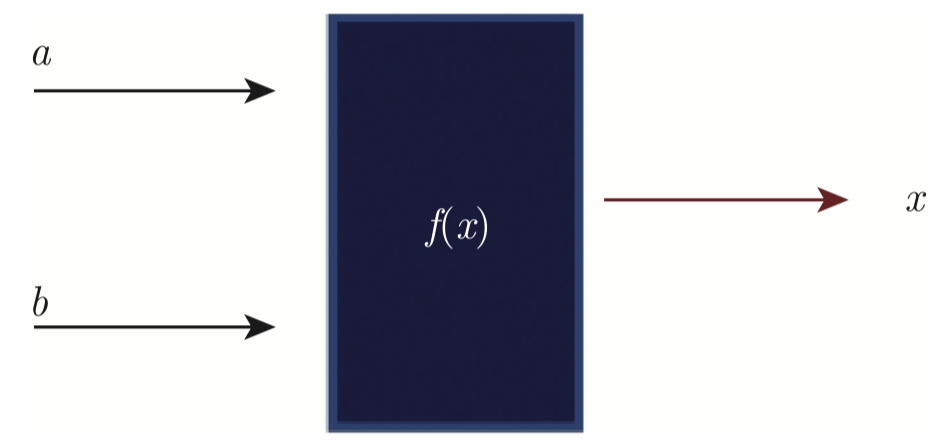
\includegraphics[width=3in]{figures/经典不可逆逻辑电路.png}
		\caption{经典不可逆电路}
	\end{minipage}
	\begin{minipage}{0.5\linewidth}
		\centering
		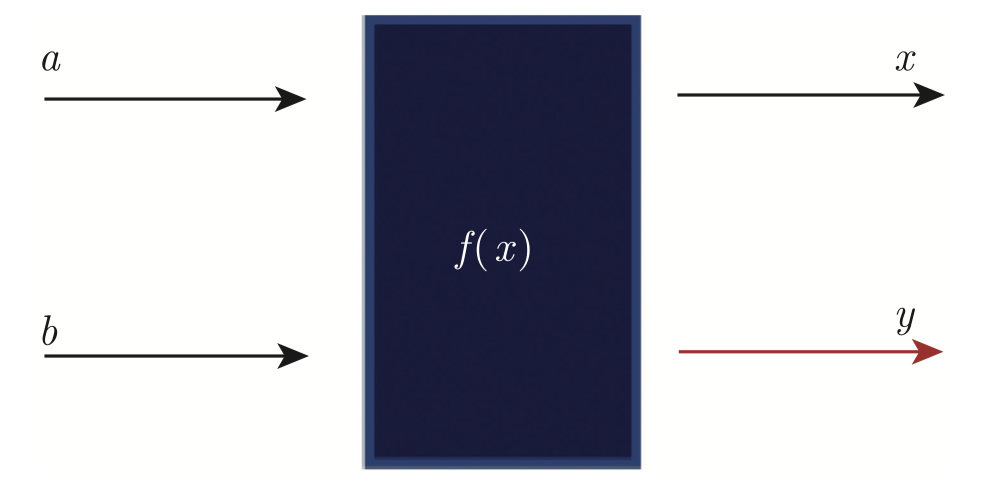
\includegraphics[width=3in]{figures/经典可逆逻辑电路.png}
		\caption{经典可逆电路}
	\end{minipage}
\end{figure}

Bennett已经证明了任何经典不可逆计算都可以转化为可逆计算的形式,而在量子计算里,酉变换构成的线路是可逆的。
经典线路不可逆计算可以通过特殊的方式转换为量子线路;通过构建黑盒子 $U_a$ 来完成可逆计算, 使用 $U_a^{-1}$ 可以复原 $|0\rangle$ 和 $|a\rangle$ 。

\begin{figure}[!htbp]
    \centering
    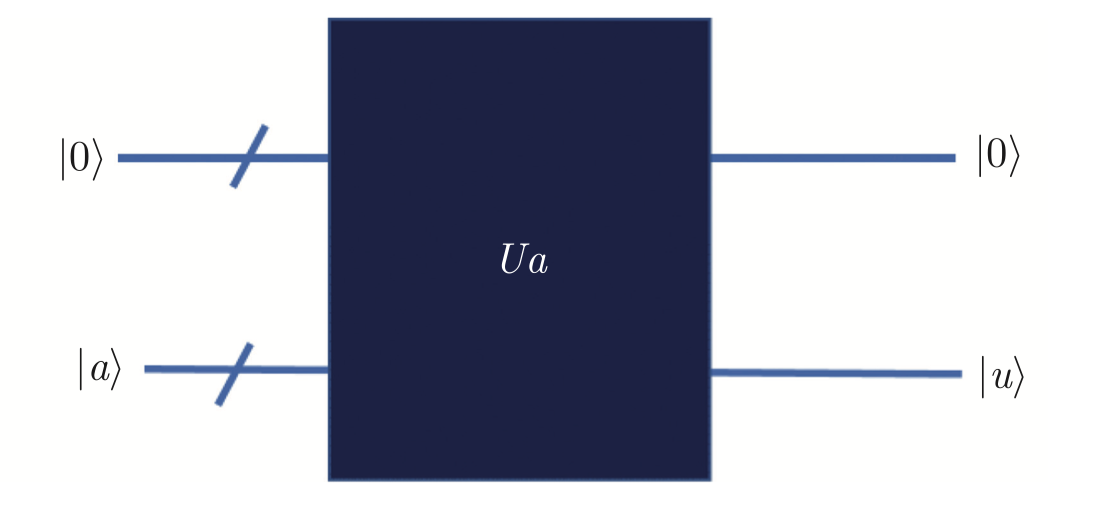
\includegraphics[width =0.45\textwidth]{figures/量子可逆线路.png}
    \caption{量子可逆线路}
\end{figure}

\subsubsection{量子加法器}
经典加法器的模型,包括了三个输入和两个输出;其中输出与输入的对应关系是:
$$
\begin{aligned}
s_i&=a_i \oplus b_i \oplus c_i \\
c_{i+1}&=a_i b_i \oplus b_i c_i \oplus a_i c_i\\
\end{aligned}
$$
\begin{figure}[!htbp]
	\begin{minipage}{0.3\linewidth}
		\centering
		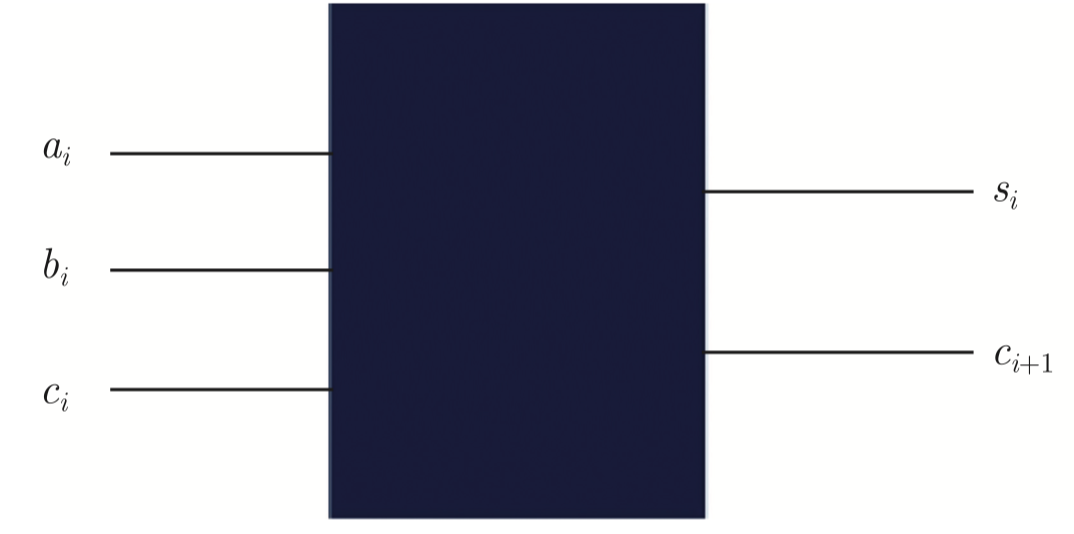
\includegraphics[width=2.5in]{figures/经典加法器模型.png}
		\caption{经典加法器模型}
	\end{minipage}
	\begin{minipage}{0.75\linewidth}
		\centering
		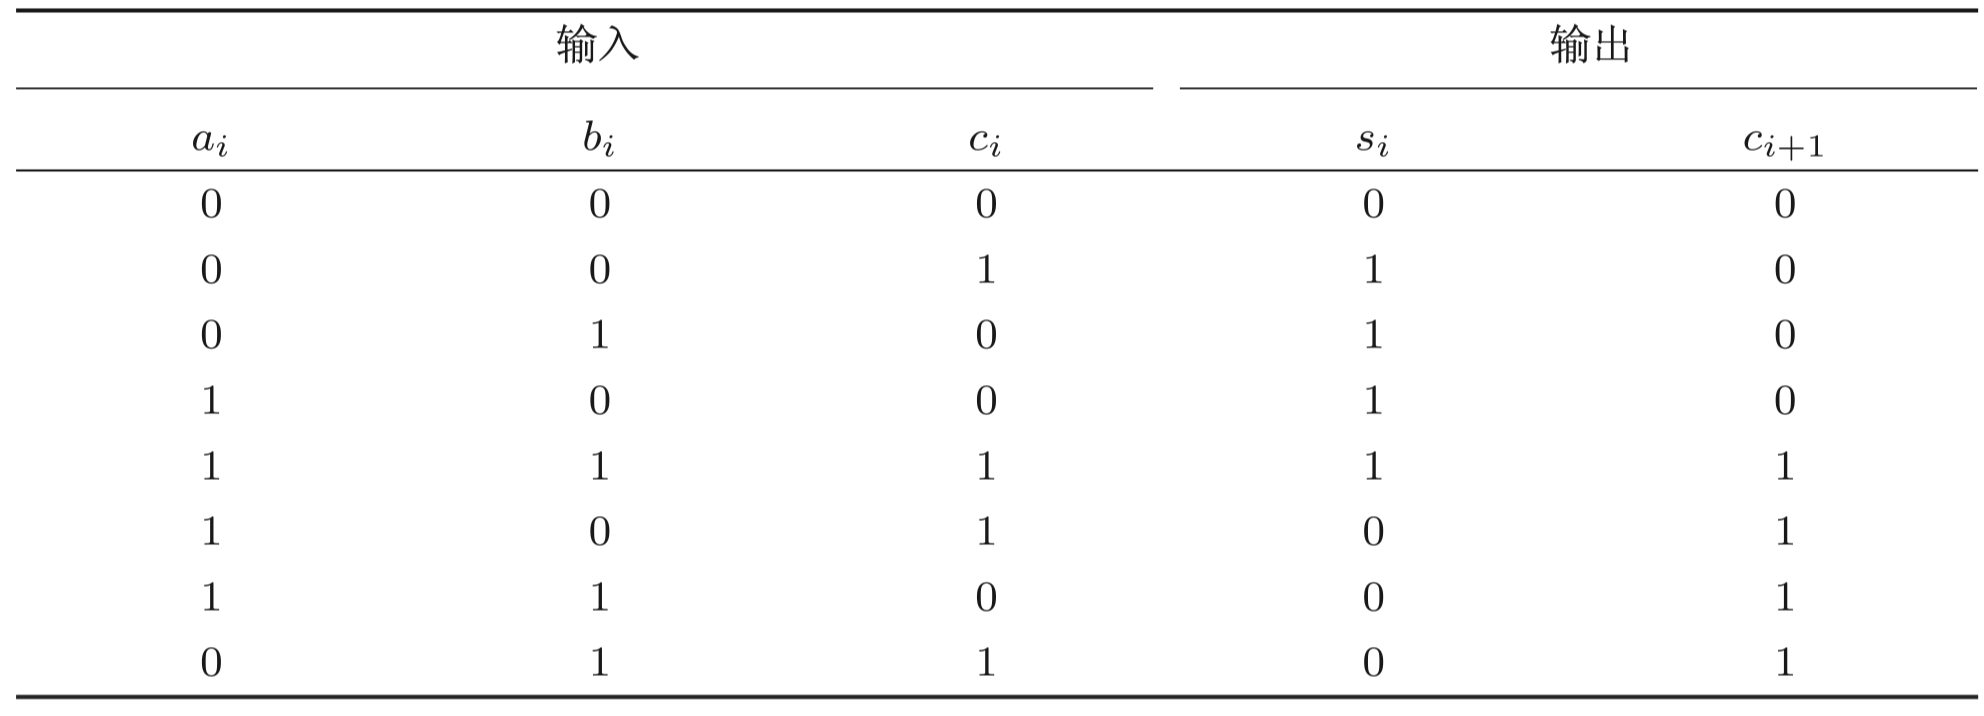
\includegraphics[width=3.5in]{figures/经典加法器真值表.png}
		\caption{经典加法器真值表}
	\end{minipage}
\end{figure}

经典加法器的模型,实际上是一个不可逆的变换,因为它有三个输入两个输出,不可实现复原操作。而量子加法器的模型需要去构建一个酉变换,不妨设置输出为:
$$
\begin{aligned}、
a_i&=a_i\\
s_i&=a_i \oplus b_i \oplus c_i \\
c_{i+1}&=a_i b_i \oplus b_i c_i \oplus a_i c_i\\
\end{aligned}
$$
\vskip -5pt
\begin{figure}[!htbp]
    \centering
    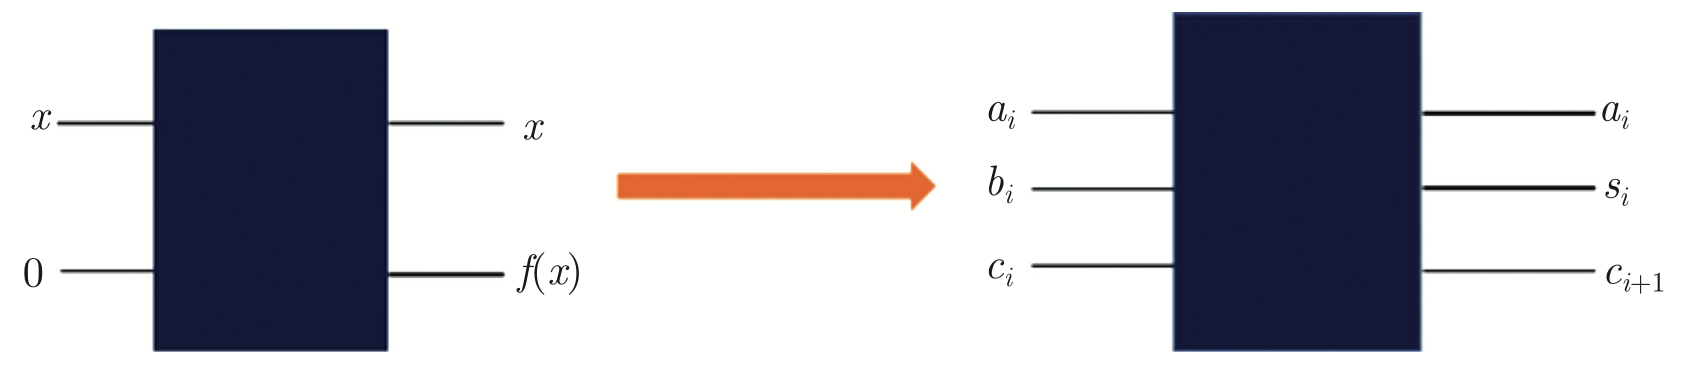
\includegraphics[width =0.9\textwidth]{figures/量子加法器模型.png}
    \caption{量子加法器模型}
\end{figure}
这样的酉变换通过MAJ模块与UMA模块实现。  
\begin{figure}[!htbp]     
    \centering     
    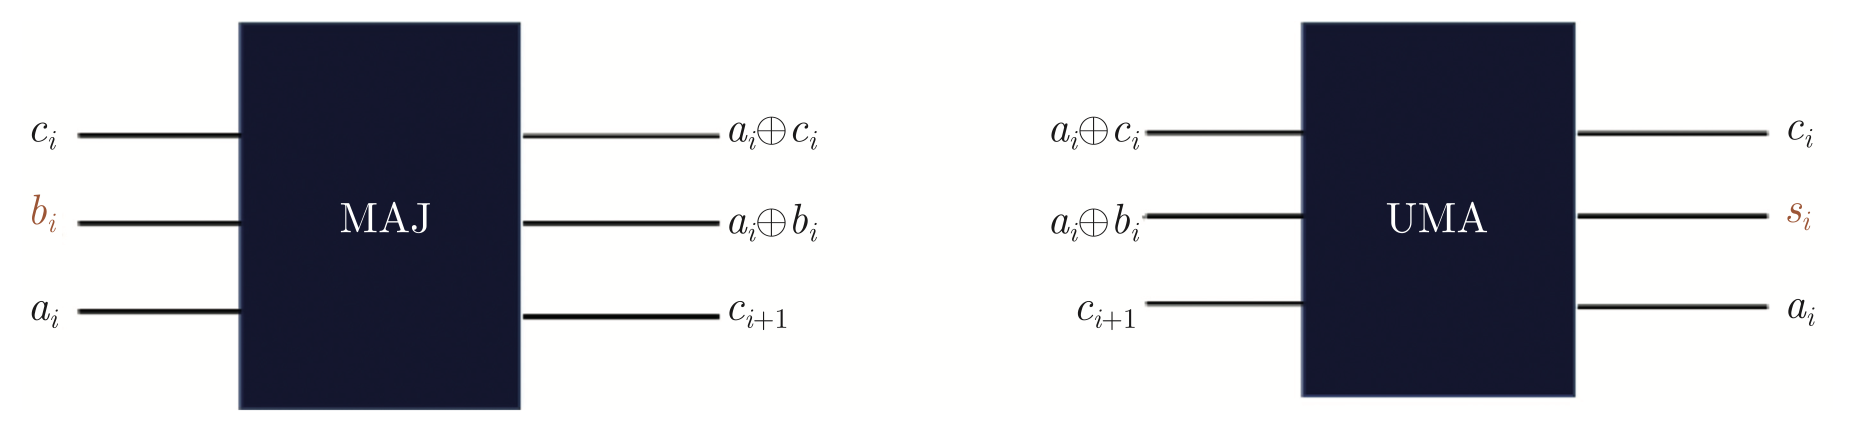
\includegraphics[width =0.9\textwidth]{figures/MAJ模块和UMA模块.png}     
    \caption{MAJ模块和UMA模块} 
\end{figure}

MAJ与UMA以一种递进的形式构建量子加法器,以$i=3$为例,给定一个初始辅助比特$c_0$和$0$,通过一系列MAJ模块得到$s_i$,再通过一系列UMA模块还原比特$c_0$。

\newpage
\begin{figure}[!htbp]     
    \centering     
    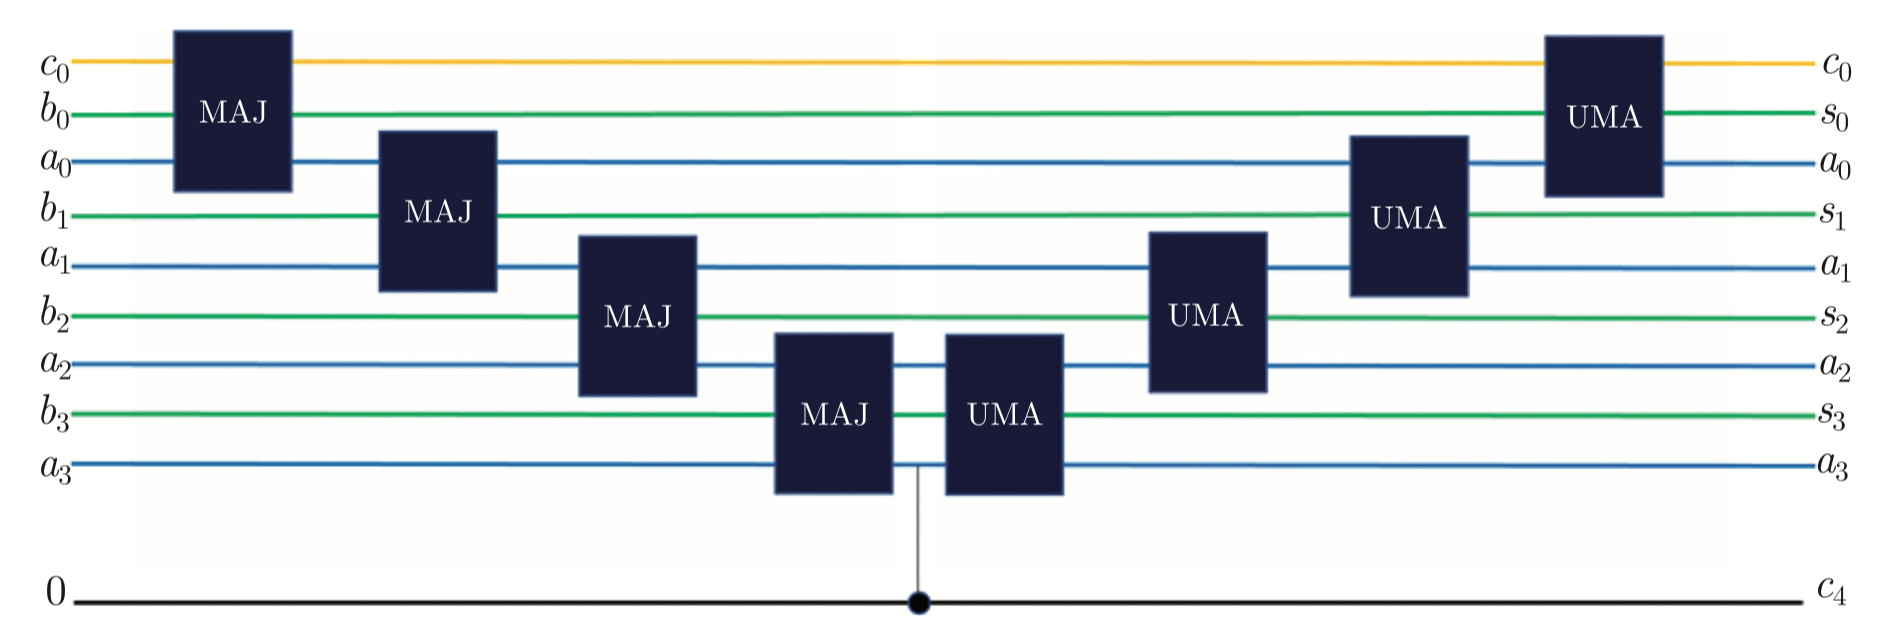
\includegraphics[width =0.75\textwidth]{figures/MAJ-UMA量子加法器.png}     
    \caption{MAJ-UMA量子加法器} 
\end{figure}

\subsubsection{量子加法器电路}
量子线路由量子逻辑门构成,量子加法器主要使用CNOT门和Toffoli门。
\vskip 8pt
\textbf{CNOT门:}$a$为控制位,$b$为受控位。$a$不变;若$a=\ket{1}$,则$b$变为$a\oplus b$。
\vskip 3pt
\textbf{Toffoli门:}$a,b$为控制位,$c$为受控位。$a,b$不变;若$a=b=\ket{1}$,则$c$变为$c\oplus ab$。

\begin{figure}[!htbp]     
    \centering     
    \includegraphics[width =0.5\textwidth]{figures/CNOT和Toffoli.png}     
\end{figure}

做变换:$c_{i+1}  =a_i b_i \oplus b_i c_i \oplus c_i a_i =a_i \oplus a_i a_i \oplus a_i b_i \oplus b_i c_i \oplus c_i a_i  =a_i \oplus\left(a_i \oplus c_i\right)\left(a_i \oplus b_i\right)$.

\noindent
整理得MAJ的电路和UMA的电路如下:

\begin{figure}[!htbp]
	\begin{minipage}{0.5\linewidth}
		\centering
		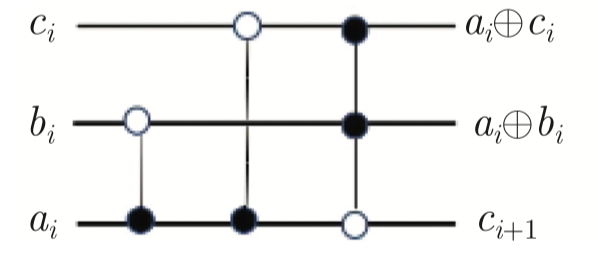
\includegraphics[width=2in]{figures/MAJ门电路.png}
		\caption{MAJ电路}
	\end{minipage}
	\begin{minipage}{0.5\linewidth}
		\centering
		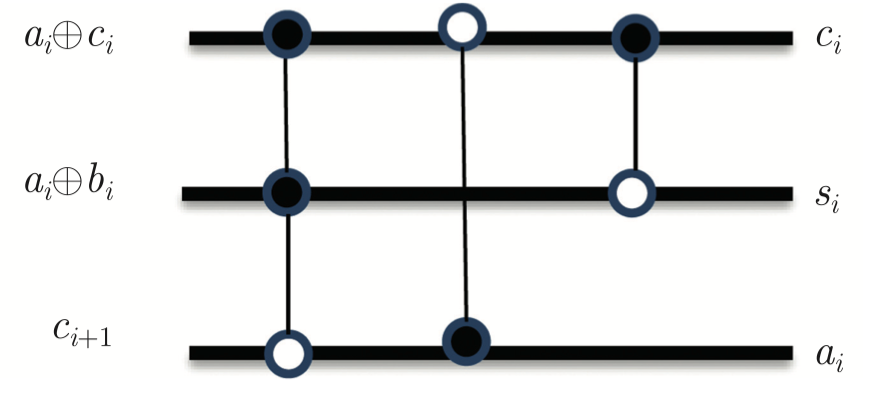
\includegraphics[width=2in]{figures/UMA门电路.png}
		\caption{UMA电路}
	\end{minipage}
\end{figure}
\begin{figure}[!htbp]     
    \centering     
    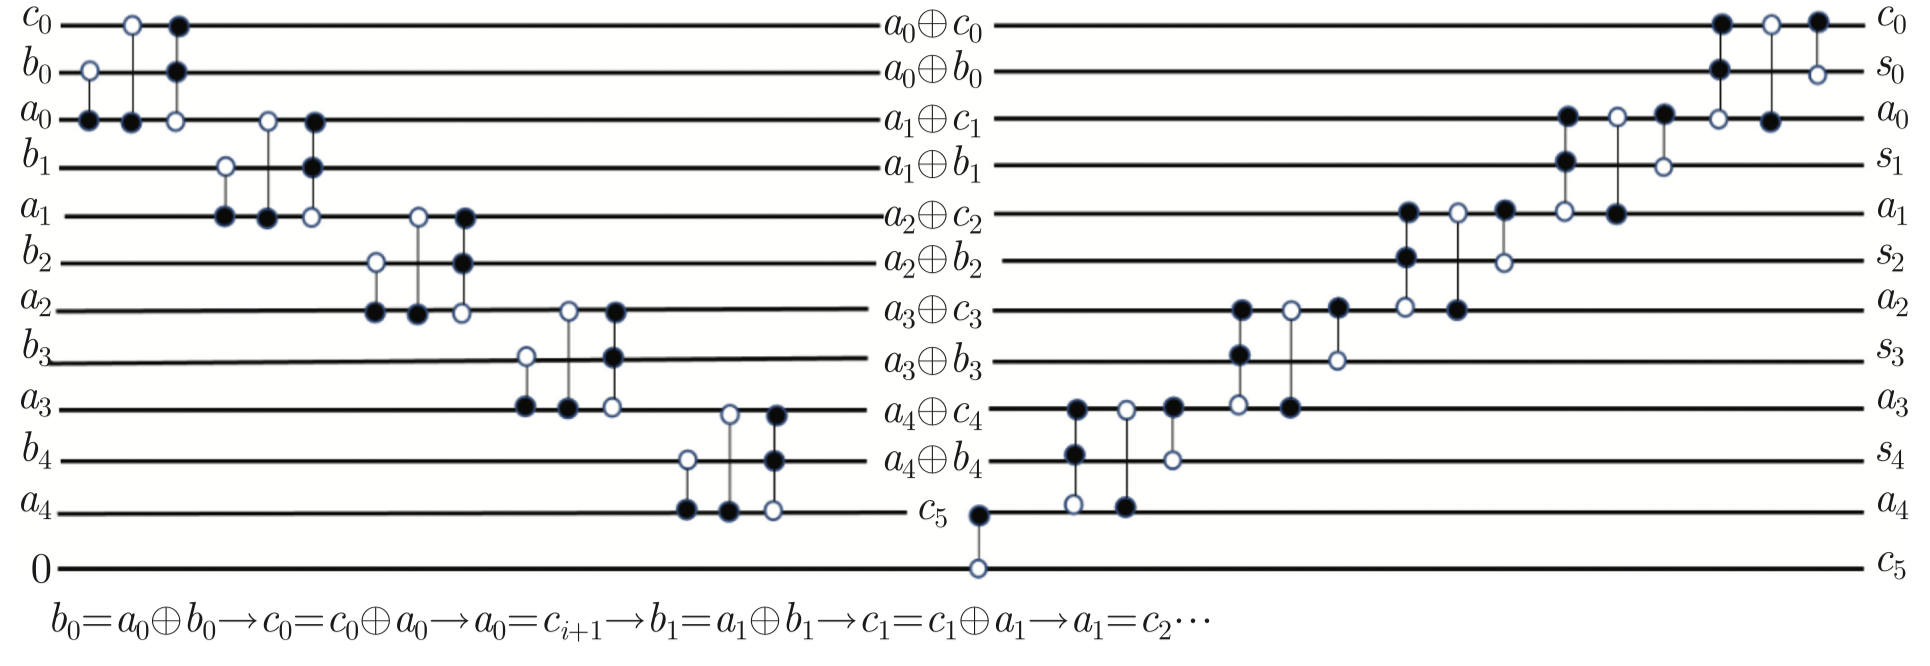
\includegraphics[width =0.69\textwidth]{figures/加法器电路.png}     
    \caption{量子加法器电路(以i=4为例)}
\end{figure}

\newpage

\subsubsection{量子傅里叶变换}
离散傅里叶变换是作用在复 $\mathrm{N}$维欧氏空间 $C^N$ 上的一个酉变换, 当输入为复向量 $\left(x_0, x_1, \cdots, x_{N-1}\right)$ 时, 其输出为复向量 $\left(y_0, y_1, \cdots, y_{N-1}\right)$, 其中:
$$
y_k=\frac{1}{\sqrt{N}} \sum_{i=0}^{N-1} x_j e^{\frac{2 \pi j i k}{N}}(k=0,1, L, N-1)
$$
量子傅里叶变换是作用在 $C^{2 N}$ 空间上的离散傅里叶变换,用量子力学表达形式为:
$$
\sum_j \alpha_j|j\rangle \rightarrow \sum_k \tilde{\alpha}_k|k\rangle
$$
其中$\tilde{\alpha}_k$的定义形式为:
$$
\tilde{\alpha}_k=\frac{1}{\sqrt{N}} \sum_{j=0}^{N-1} e^{2 \pi i j k / N} \alpha_j
$$
从线性算子的角度,对应的矩阵为酉矩阵:
$$
\mathrm{QFT}=\frac{1}{\sqrt{M}}\left(\begin{array}{cccccc}
1 & 1 & 1 & 1 & \cdots & 1 \\
1 & \omega & \omega^2 & \omega^3 & \cdots & \omega^{M-1} \\
1 & \omega^2 & \omega^4 & \omega^6 & \cdots & \omega^{2 M-2} \\
\vdots & \vdots & \vdots & \vdots & \ddots & \vdots \\
1 & \omega^{M-1} & \omega^{2 M-2} \omega^{3 M-3} & \cdots & \cdots & \omega^{(M-1)(M-1)}
\end{array}\right)
$$
由此可见,量子傅里叶变换是可逆的酉变换。

\vskip 10pt
考虑正整数的二进制表示:
$$
\begin{aligned}
j_1 j_2 \cdots j_n&=j_1 2^{n-1}+j_2 2^{n-2}+\cdots+j_n\\
0 . j_l j_{l+1} \cdots j_m&=\frac{j_l}{2}+\frac{j_{l+1}}{4}+\cdots+\frac{j_m}{2^{m-l+1}}\\
\end{aligned}
$$
则量子傅里叶变换可表示为:
$$
\ket{j_1 \cdots j_n}\rightarrow
\frac{\left(|0\rangle+e^{2 \pi i 0 . j_n}|1\rangle\right)\left(|0\rangle+e^{2 \pi i 0 . j_{n-1} j_n}|1\rangle\right) \cdots\left(|0\rangle+e^{2 \pi i 0 . j_1 j_2 \cdots j_n}|1\rangle\right.}{2^{n / 2}}
$$

\subsubsection{量子傅里叶变换电路}
量子傅里叶变换主要由Hadamard门和CR门构成。

\vskip 5pt
(1)Hadamard门的矩阵形式是一个 $2 \times 2$ 的酉矩阵:
$$
H=\frac{1}{\sqrt{2}}\left(\begin{array}{cc}
1 & 1 \\
1 & -1
\end{array}\right)
$$

$\quad\;\cdot$ 对于 $|0\rangle: H|0\rangle=\frac{1}{\sqrt{2}}(|0\rangle+|1\rangle)$,

$\quad\;\cdot$ 对于 $|1\rangle: H|1\rangle=\frac{1}{\sqrt{2}}(|0\rangle-|1\rangle)$.
\newpage

%\vskip 5pt
(2)CR门在控制位为 $|1\rangle$ 时做控制相位变换操作, 受控运算符的矩阵形式为:
$$
\hat{R}_k=\left(\begin{array}{cc}
1 & 0 \\
0 & e^{2 \pi i / 2^k}
\end{array}\right)
$$

$\quad\;\cdot$ 当控制位为 $|0\rangle$ 时,受控位保持不变,

$\quad\;\cdot$ 当控制位为 $|1\rangle$ 时,受控位的相位会绕相位轴旋转 $\frac{\pi}{2^{k-1}}$ 角度。

\vskip 5pt
通过一系列Hadamard门和CR门即可实现量子傅里叶变换电路
\begin{figure}[!htbp]     
    \centering     
    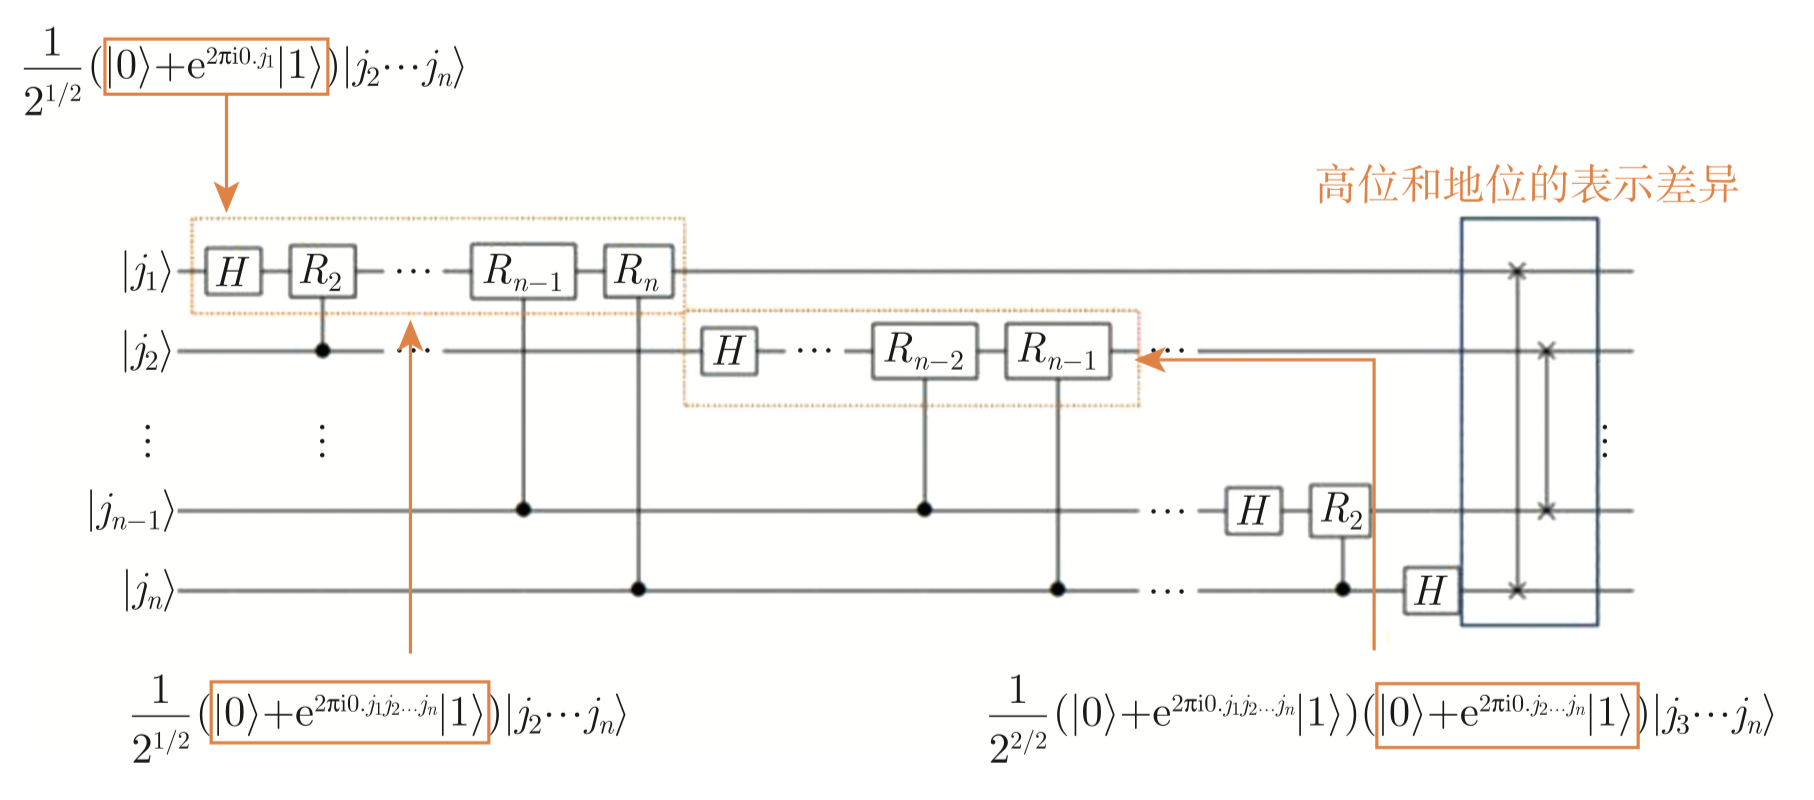
\includegraphics[width =0.9\textwidth]{figures/量子傅里叶变换电路.png}     
    \caption{量子傅里叶变换电路}
\end{figure}

如果初始化都是0,则控制不工作,线路等价于对所有比特做Hadamard门操作。

\subsection{Shor算法的原理}
\subsubsection{算法原理概述}
从时间上比较,Shor算法可以将素数分解的最佳复杂度大幅降低

\begin{figure}[!htbp]
	\begin{minipage}{0.5\linewidth}
		\centering
		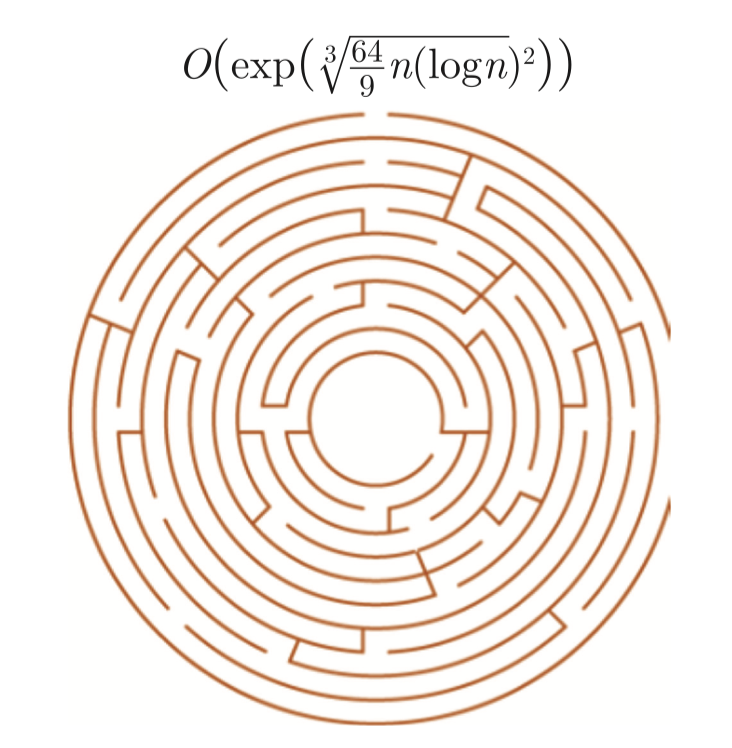
\includegraphics[width=2in]{figures/传统素数分解.png}
		\caption{传统素数分解的最佳复杂度}
	\end{minipage}
	\begin{minipage}{0.5\linewidth}
		\centering
		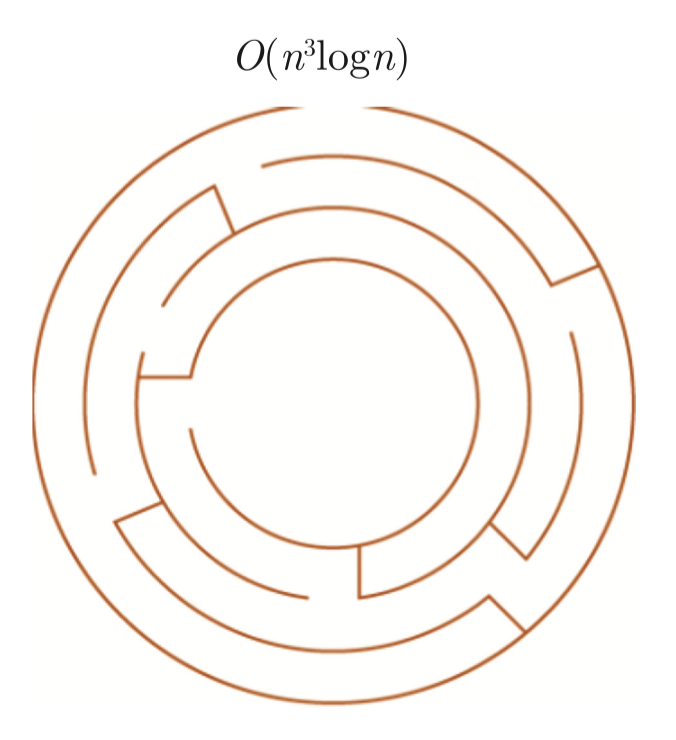
\includegraphics[width=1.85in]{figures/Shor算法分解.png}
		\caption{Shor算法的复杂度}
	\end{minipage}
\end{figure}

Shor算法的思想, 是将分解问题转化为寻找模指数电路的周期问题, 构建模指数电路, 通过逆 QFT找到模指数电路的周期。
Shor 算法的核心电路主要包含傅里叶变换 (QFT), 模指线路 $U_{\mathrm{f}}$ 计算函数, 以及逆傅里叶变换 $\left(\mathrm{QFT}^{-1}\right)$ 。

\begin{figure}[!htbp]     
    \centering     
    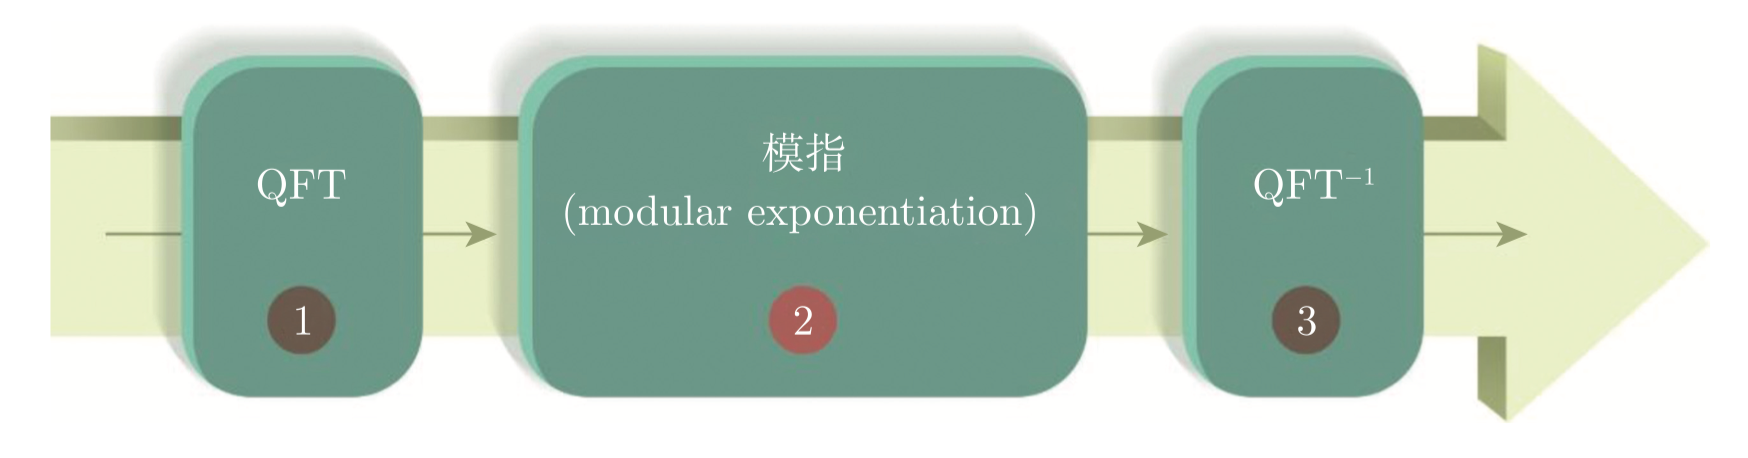
\includegraphics[width =0.65\textwidth]{figures/Shor算法的核心电路.png}     
    \caption{Shor算法的核心电路}
\end{figure}

\subsubsection{问题转化}
假设分解的数为 $\mathrm{N}$, 任取 $a \in[2, N-1]$, 满足 $\mathrm{a}$ 和 $\mathrm{N}$ 互质,且
$$
\begin{array}{l}
a^r=1 \bmod N \quad \text { (其中 } \mathrm{r} \text { 为偶数) } \\
\left(a^{\frac{r}{2}}+1\right)\left(a^{\frac{r}{2}}-1\right)=k N
\end{array}
$$
如果
$$
a^{\frac{r}{2}} \neq-1 \bmod N, a^{\frac{r}{2}} \neq 1 \bmod N
$$
得到 $\mathrm{N}$ 的两个因子 $p_1$ 和 $p_2$
$$
p_1=\operatorname{gcd}\left(a^{\frac{r}{2}}+1, N\right) \text { 和 } p_2=\operatorname{gcd}\left(a^{\frac{r}{2}}-1, N\right)
$$
注意到如果 $N=p^m$, 则无法用该方法进行转化, 所以在算法开始之 还需做如下判定: 判断 $\sqrt[k]{N} \in Z$ 是否为真, 其中 $k \leq \log 2 N$.

\subsubsection{算法电路}
Shor算法电路框架总共包括四个板块,分别是模指模块、常数模乘、常数模加、以及加法器的构造。

\begin{figure}[!htbp]     
    \centering     
    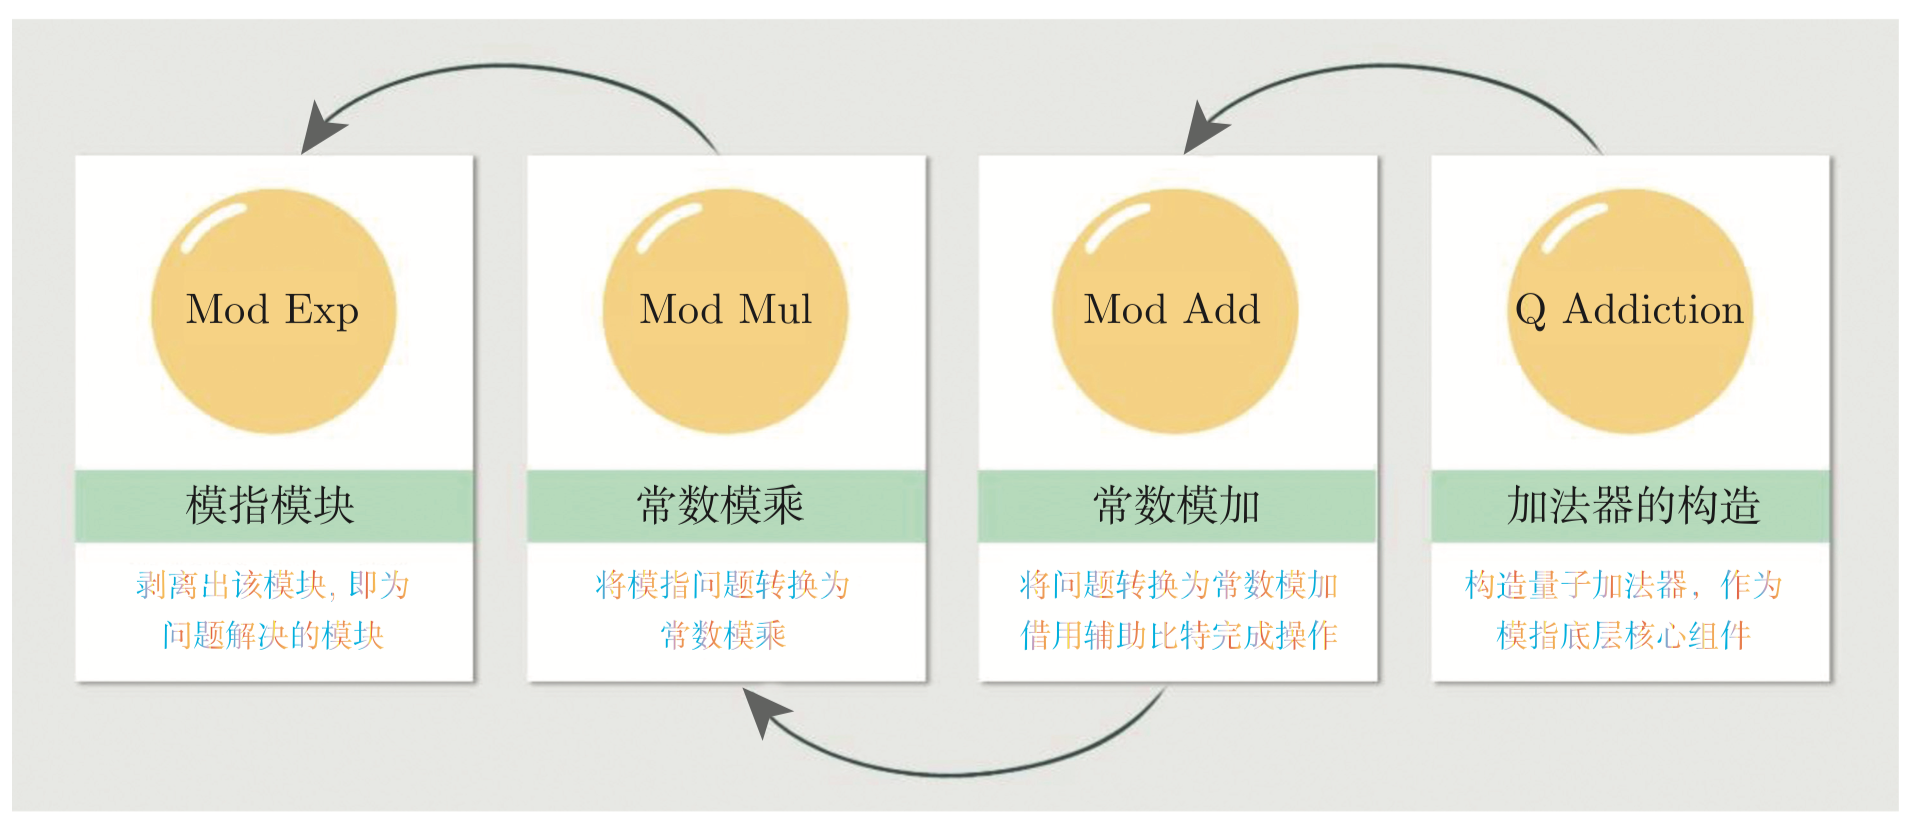
\includegraphics[width =0.63\textwidth]{figures/Shor算法电路框架.png}     
    \caption{Shor算法电路框架}
\end{figure}
\newpage

\noindent
量子加法器是模指底层的核心组件;通过加法器的构造来构建常数模加,借用辅助比特完成操作;再由常数模加来构建常数模乘,将模指问题转换为可求解的模常数模块;再由常数模乘来完成最终的模指模块。

Shor算法的量子线路图如下所示,接下来我们将对各部分电路进行详细分析。

\begin{figure}[!htbp]     
    \centering     
    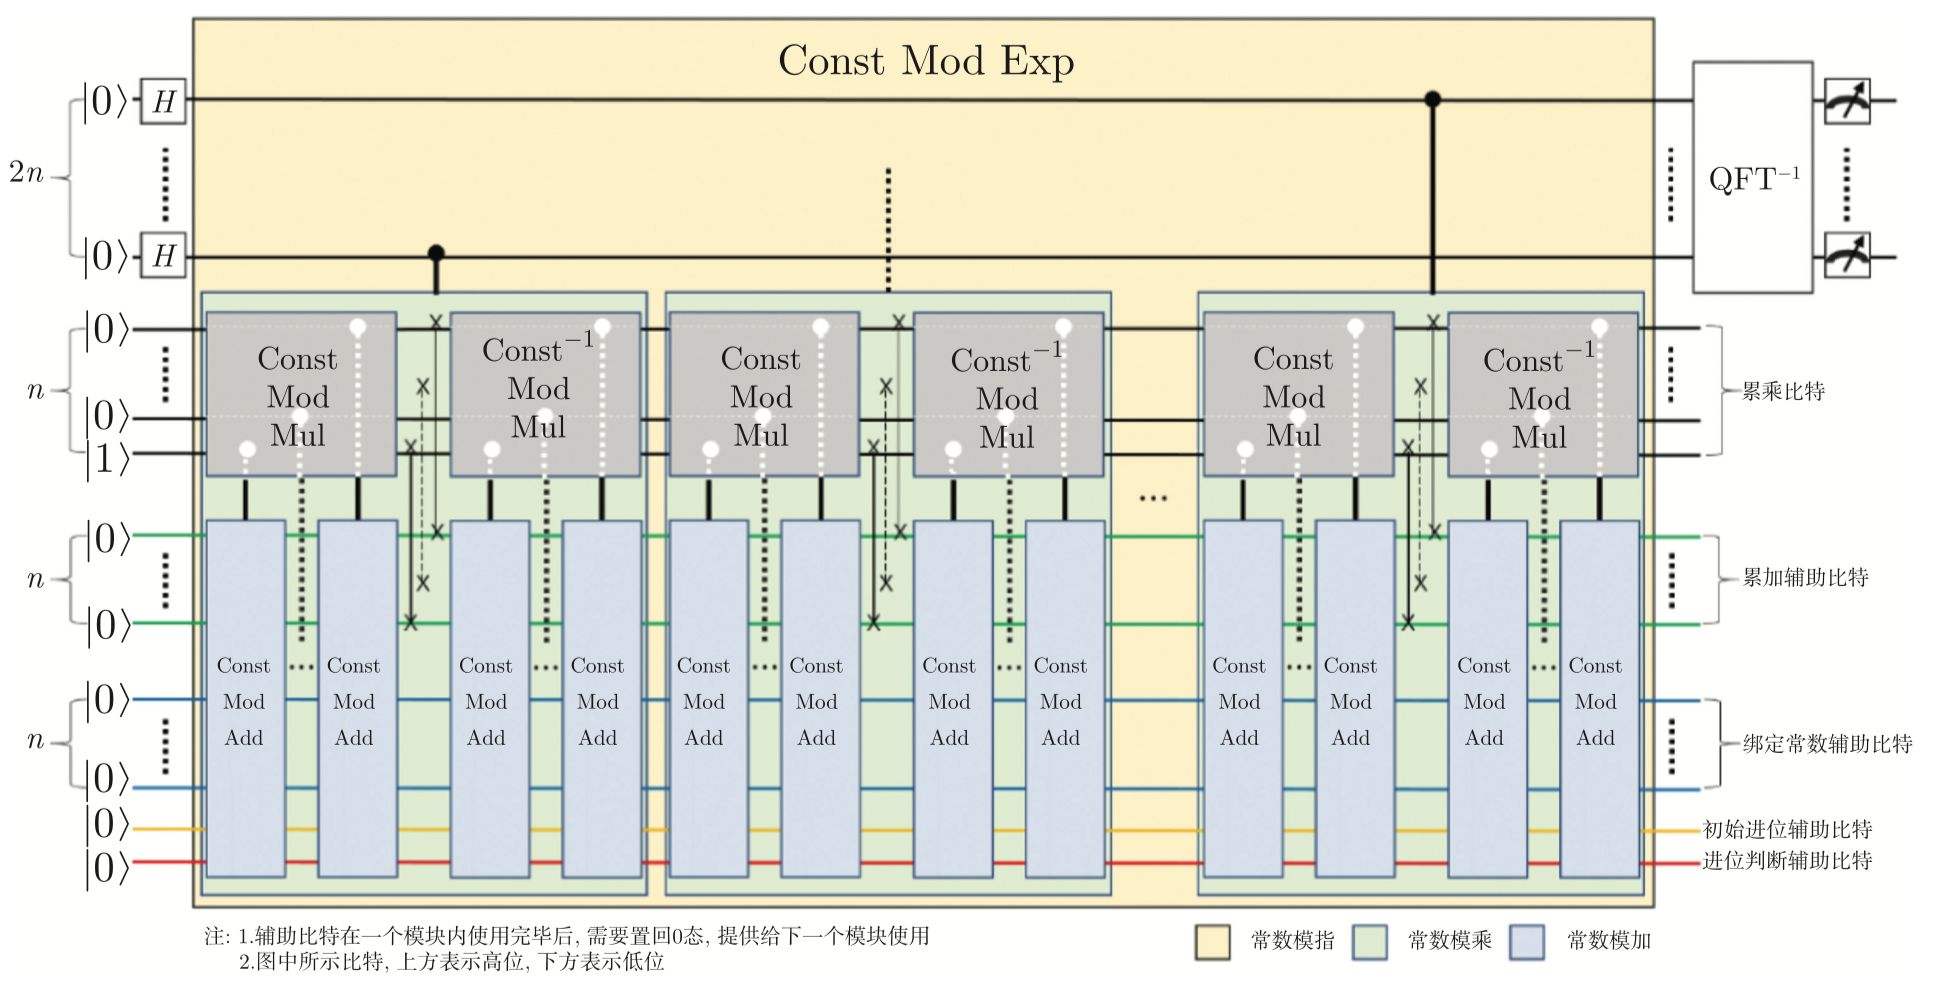
\includegraphics[width =0.95 \textwidth]{figures/Shor算法电路.png}     
    \caption{Shor算法电路}
\end{figure}

\noindent
\textbf{Step 1. 模指模块}
\vskip 10pt

QFT和模指数电路 $f(x)=a^x \bmod N$
$$
|x\rangle|1\rangle \rightarrow|x\rangle|f(x)\rangle
$$
$\mathrm{N}$ 对应的二进制长度为 $n$, 输入的 $x$ 的位数 $m$ 不固定, 一般为 $2 n$ 位, 即 $m=2 n$; 考虑 $\left[\log _2 N\right]$ 是分解数 $\mathrm{N}$ 所需要表示的比特数。

\vskip 10pt
\noindent
\textbf{Step 2. 常数模乘}
\vskip 10pt

模指: $f(x)=a^x \bmod N, \mathrm{x}$ 的二进制表达方式如下:
$$
\mathrm{x}=\left(\mathrm{x}_{2 \mathrm{n}-1}, \cdots, x_1, \mathrm{x}_0\right)=\sum_{i=0}^{2 n-1} x_i \times 2^i
$$
其中
$$
X_i,(i=0 \ldots 2 n-1)
$$
$f(x)$ 可以写成
$$
f(x)=\prod_{i=0}^{t-1} a^{2^i x_i} \bmod N=a^{x_i \times \sum_i^{2 n-1} a^i} \bmod N
$$
即:
$$
\left(\mathrm{a}^{2^0} \bmod N\right)^{x_0} \cdot\left(a^{2^1} \bmod N\right)^{x_1} \cdots\left(a^{2^{2 n-1}} \bmod N\right)^{x_{2 n-1}} \bmod N
$$
假设有电路 $U|y\rangle \rightarrow \mid C y \bmod N)$, 取 $C$ 为 $a^{2^i}, i=0,1, \ldots, 2 n-1$, 将 $|y\rangle$ 的初态设为 $|1\rangle$, 然后依次经过 $C_i U_i$ 门 :
$$
|1\rangle \rightarrow\left|a^{x_i \times \sum_i^{2 n-1} a^i}\right\rangle \sim \sim\left|a^x \bmod N\right\rangle
$$
这里总共有 $2 \mathrm{n}$ 个控制 $\mathrm{U}$ 块。每个输入量子比特都控制着下方的模 $\mathrm{N}$ 乘法器 $\mathrm{CU}_{\mathrm{a}^{2^i}}$ 
首先在 $|x\rangle$ 上加 $Q F T$ 构成叠加态, 同时将 $2^{2 n-1}$ 个 $x$ 输入电路, 用 $Q F T^{-1}$ 分析经过模 指电路后的态的周期性, 从而得到 $f(x)$ 的周期。

\begin{figure}[!htbp]     
    \centering     
    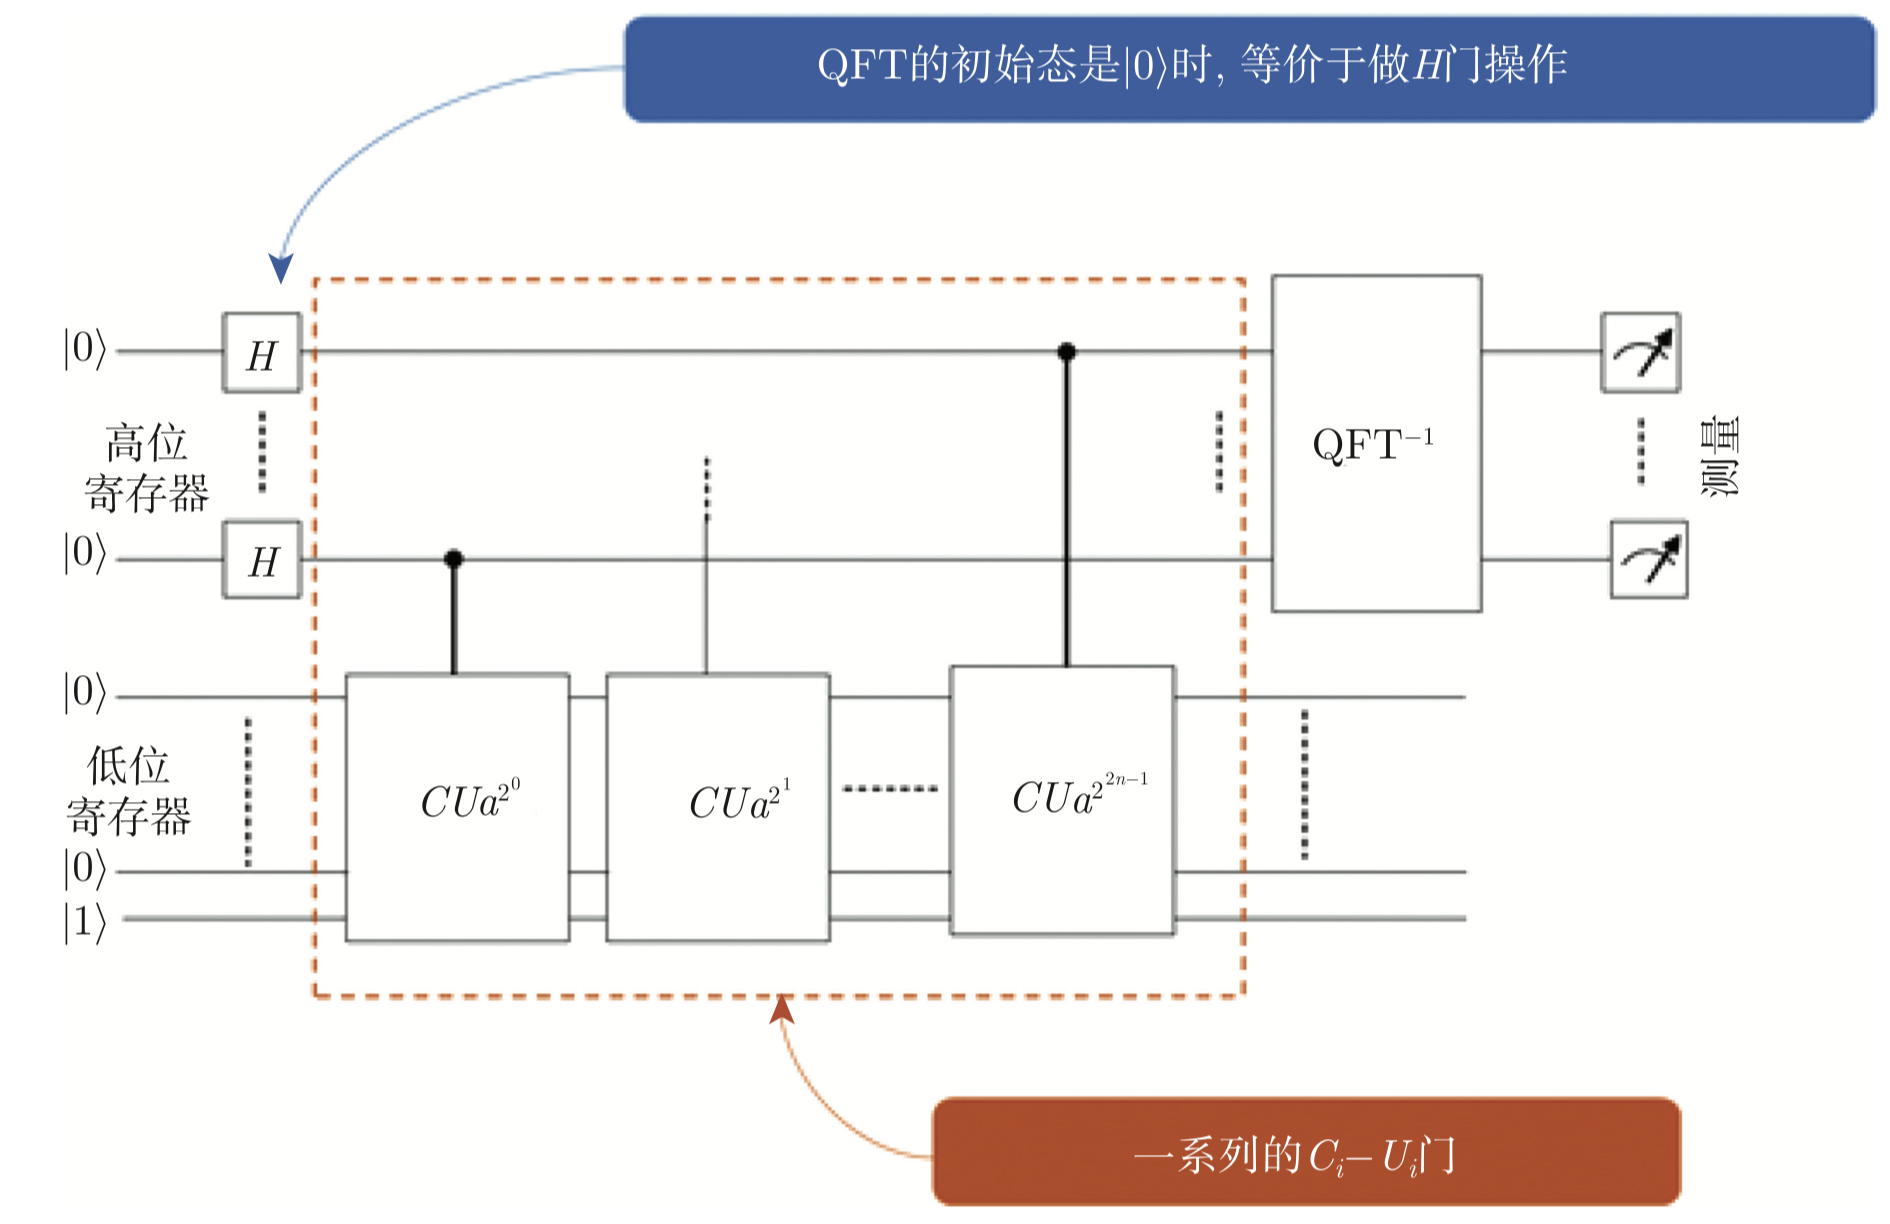
\includegraphics[width =0.7 \textwidth]{figures/常数模乘1.png}     
    \caption{常数模乘电路框架}
\end{figure}

例如: $U|y\rangle \rightarrow|C y \bmod N\rangle$ 使用同样的方法用二进制表示 $y=\sum_{i=0}^{n-1} y_i \times 2^i$ ,同理 $y_i$ 做控制位, 将所需问题转化为加法 $C_i-U(A D D)$ :
$$
|y\rangle|z\rangle \rightarrow|y\rangle\left|z+C \times 2^i\right\rangle
$$
首先, $|z\rangle$ 初态置为 $|0\rangle$, 经过一连串 $C_i-A D D$ 得到
$$
|y\rangle|0\rangle \rightarrow|y\rangle|C y \bmod N\rangle
$$
再通过交换操作 :
$$
|y\rangle|C y \bmod N\rangle \rightarrow|C y \bmod N\rangle|y\rangle
$$
最终目标:
$$
|C y \bmod N\rangle|y\rangle \rightarrow|C y \bmod N\rangle|0\rangle
$$
整个过程如图20所示:
$$
|y\rangle|0\rangle \rightarrow|C y \bmod N\rangle|0\rangle
$$

\newpage
\begin{figure}[!htbp]
	\begin{minipage}{0.5\linewidth}
		\centering
		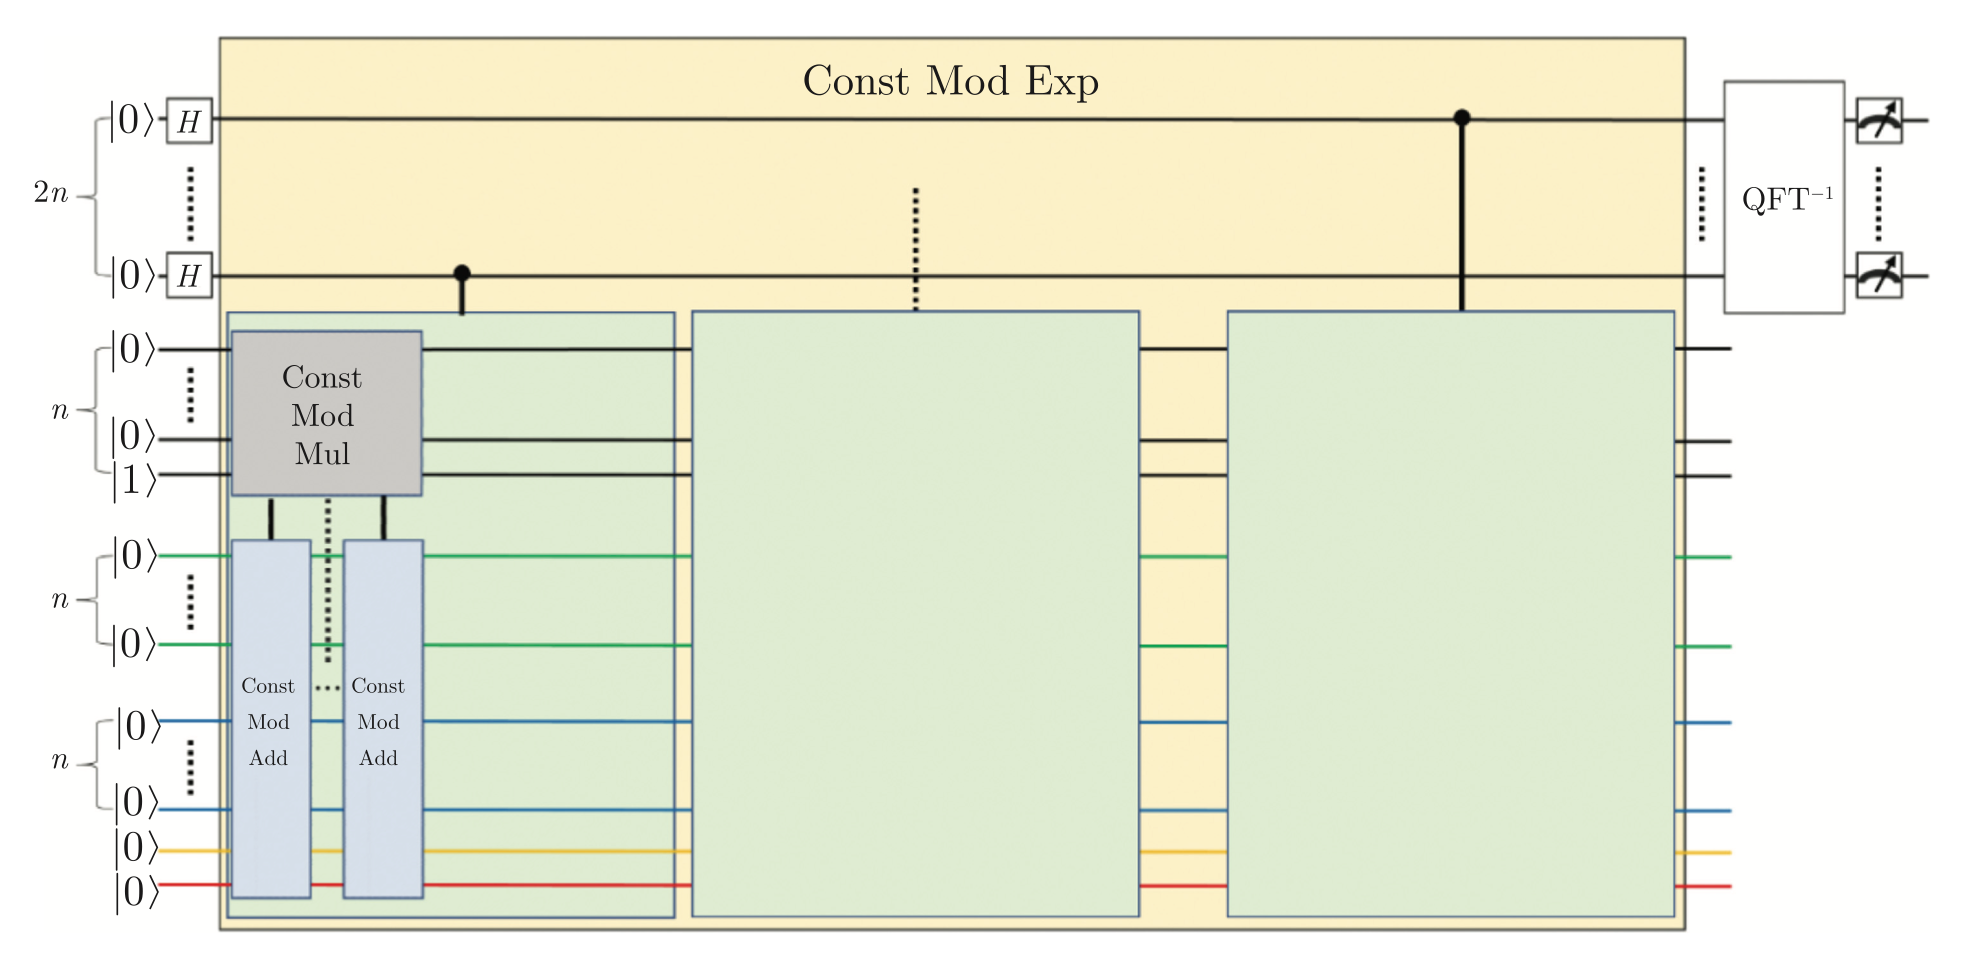
\includegraphics[width=3.4in]{figures/常数模乘2.png}
	\end{minipage}
	\begin{minipage}{0.5\linewidth}
		\centering
		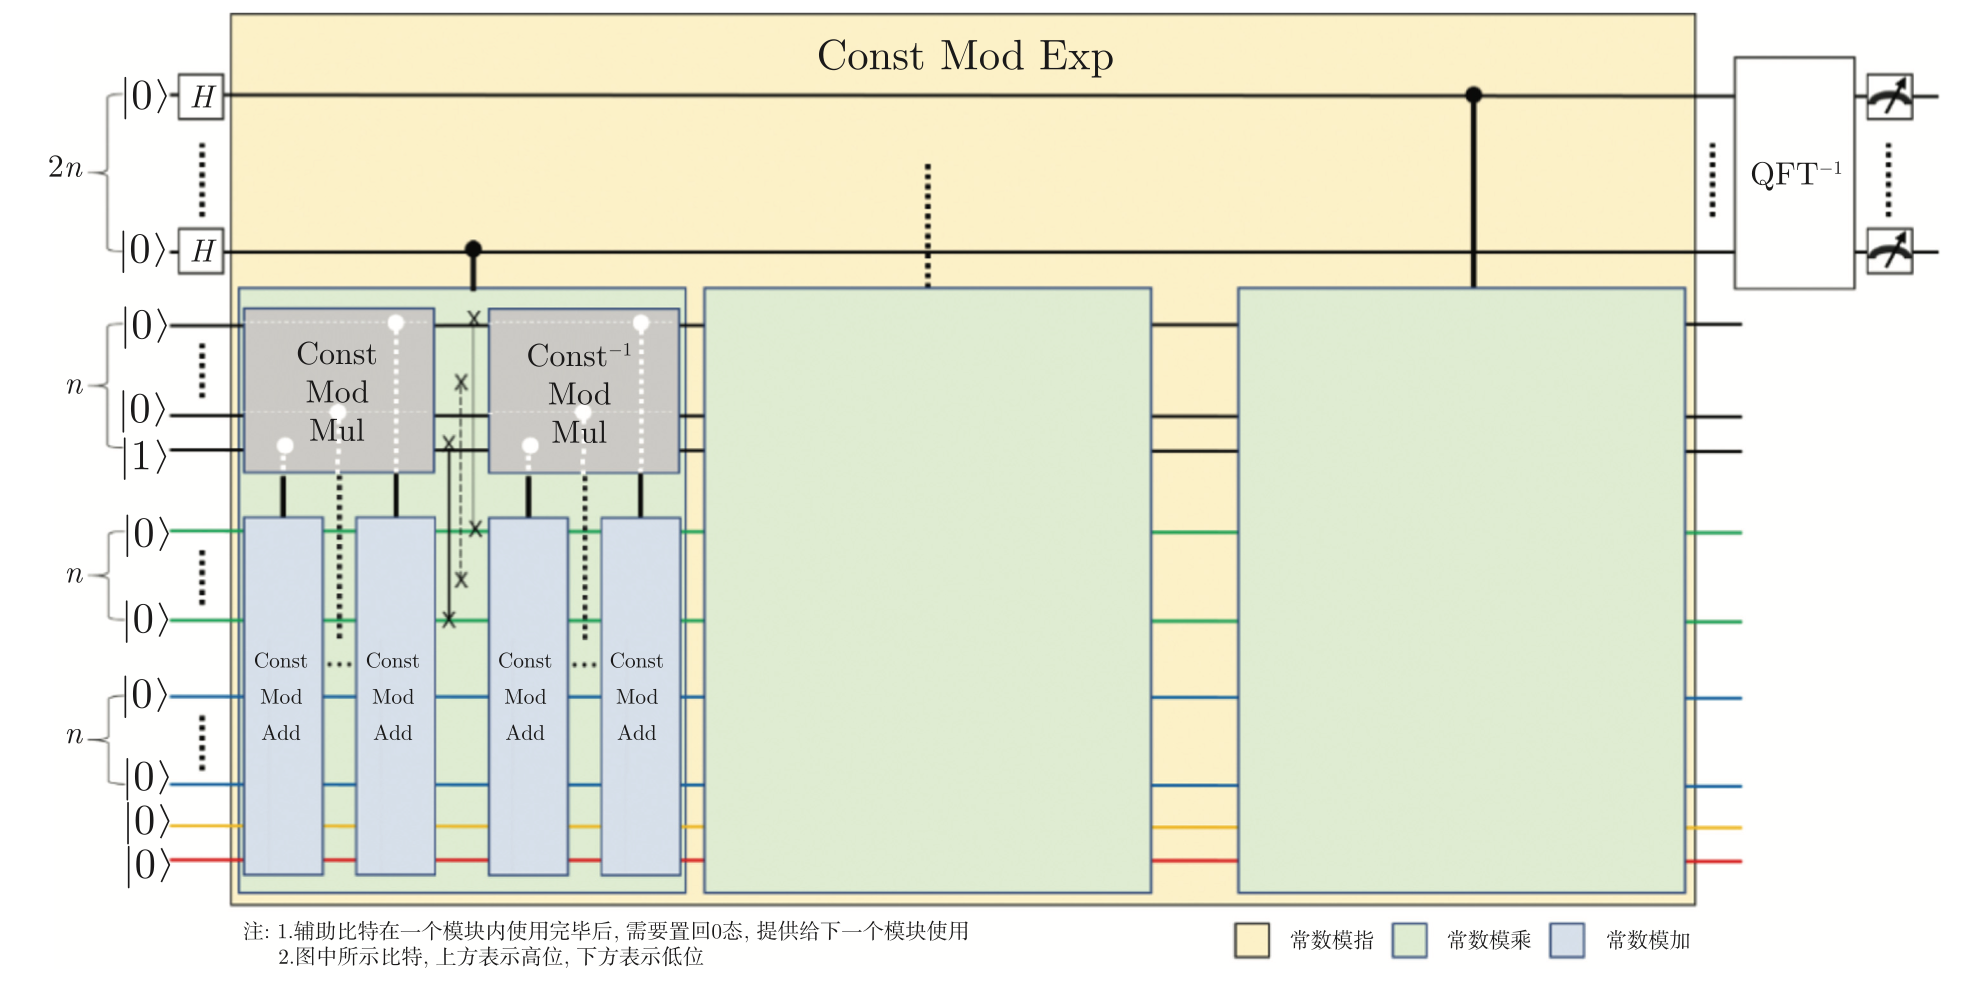
\includegraphics[width=3.4in]{figures/常数模乘3.png}
	\end{minipage}
    \caption{先转换成一组常数模加,再将常数模加中的辅助比特回收}
\end{figure}

\vskip 10pt
\noindent
\textbf{Step 3. 常数模加}
\vskip 10pt

常数模加输入 $2 N+2$ 个量子比特,其中底部有两个辅助比特, 分别是初始进位辅助比特和进位判断辅助比特。

\begin{figure}[!htbp]     
    \centering     
    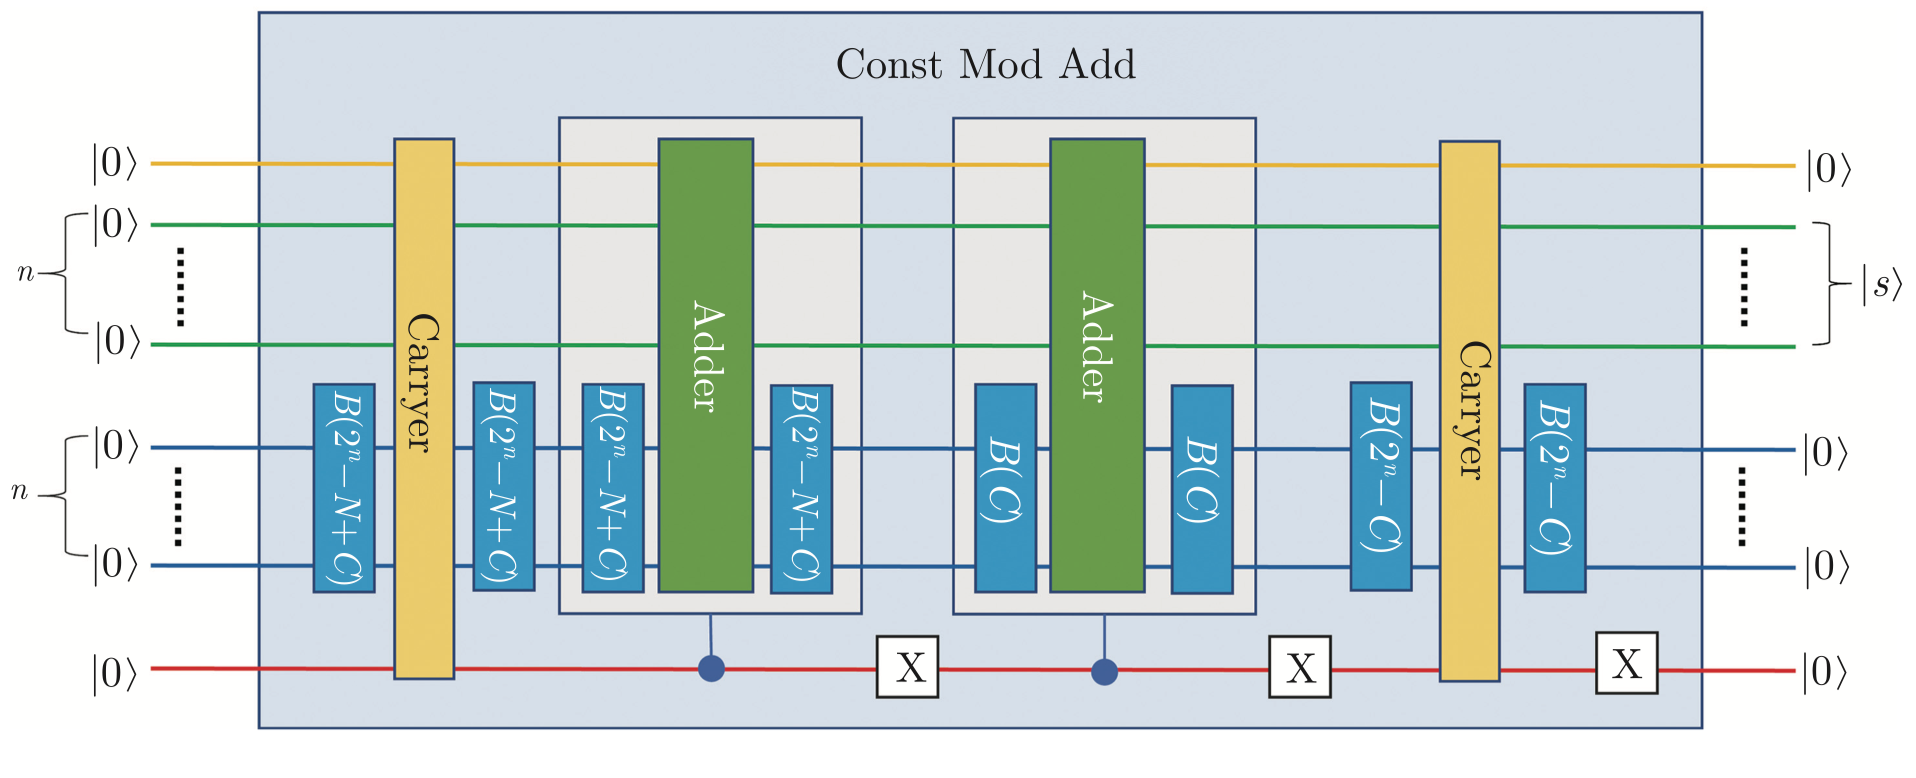
\includegraphics[width =0.7 \textwidth]{figures/常数模加电路框架.png}     
    \caption{常数模加电路框架}
\end{figure}

\noindent
常数模加内部包含的三个模块, 分别是绑定数据 (B $\left(2^n-N+C\right))$; 进位器 (Carrier) ; 加法器 (Adder),具体结构如下:

\begin{figure}[!htbp]
	\begin{minipage}{0.4\linewidth}
		\centering
		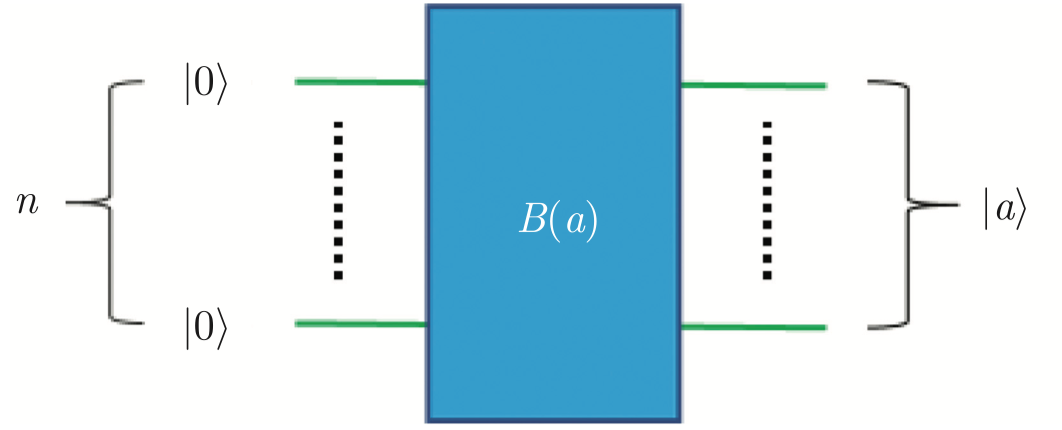
\includegraphics[width=2.3in]{figures/绑定数据.png}
	\end{minipage}
	\begin{minipage}{0.6\linewidth}
		\centering
		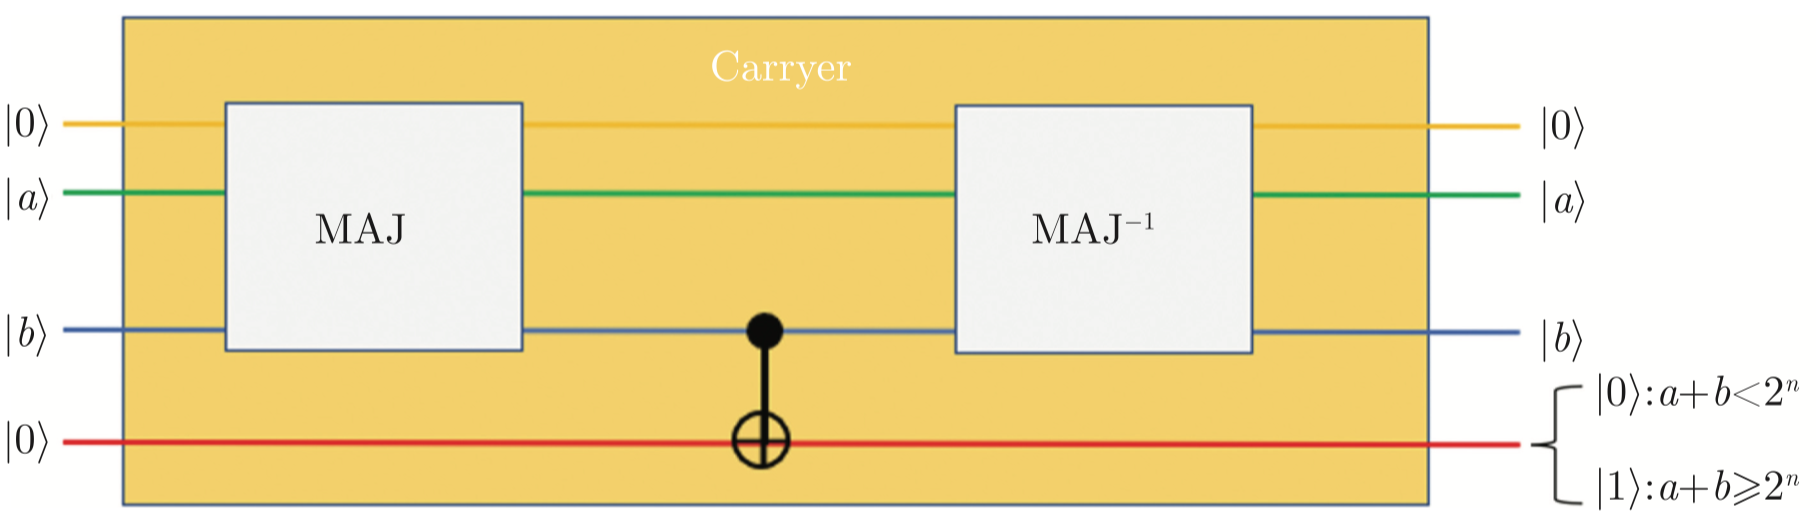
\includegraphics[width=3.4in]{figures/进位器.png}
	\end{minipage}
\end{figure}
\vskip -18pt
\begin{figure}[!htbp]     
    \centering     
    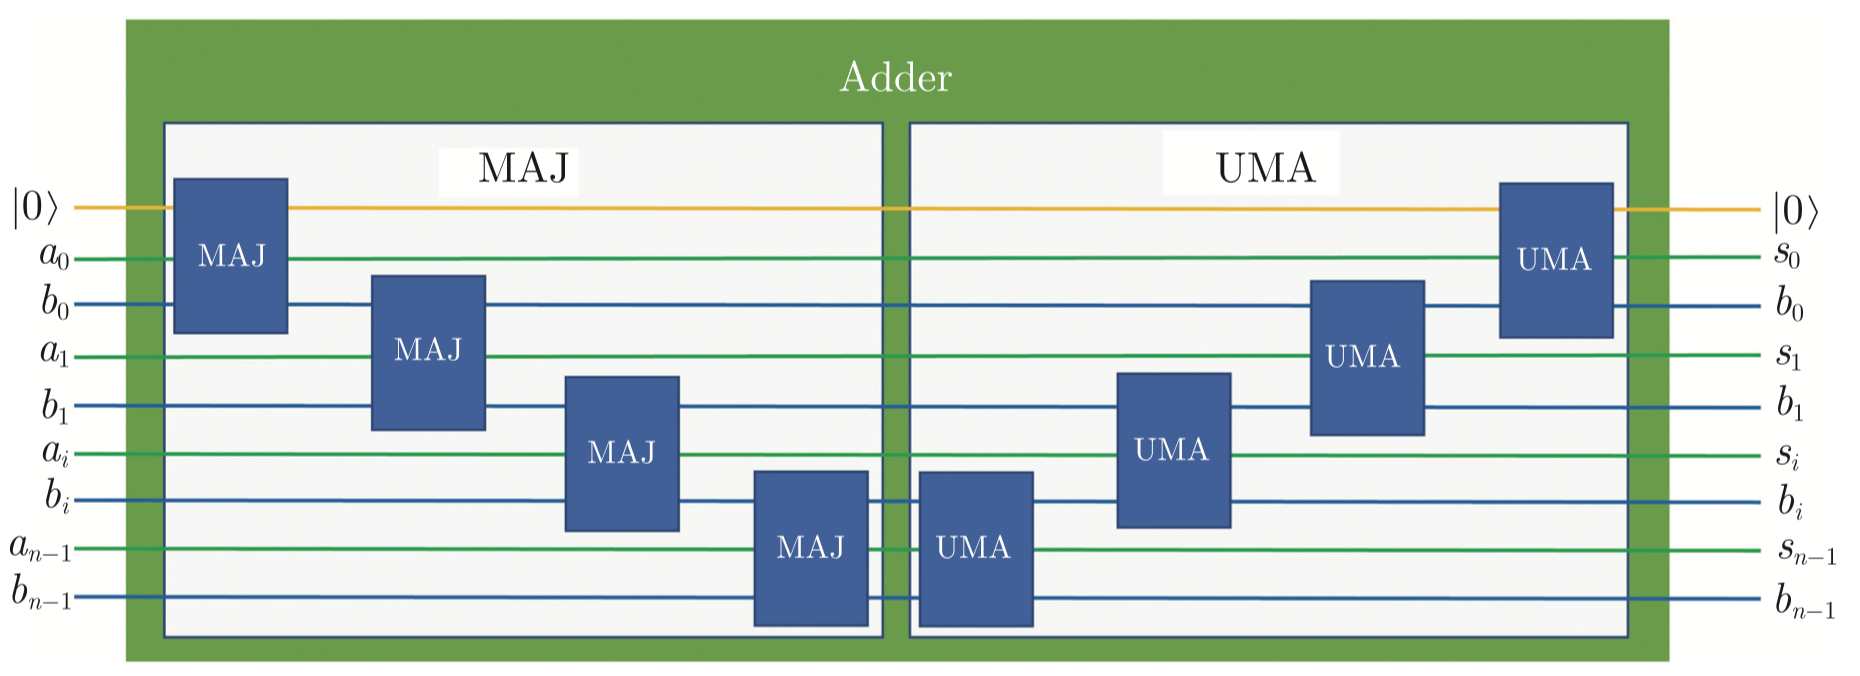
\includegraphics[width =0.6 \textwidth]{figures/加法器.png}     
    \caption{绑定数据(左上),进位器(右上),加法器(下)}
\end{figure}
\newpage

\noindent
常数模加的工作机制为:

\vskip 3pt
1. 绑定数据, 将 $\mathrm{N}$ 个初始化为 0 的输入比特绑定为 $|a\rangle$, 绑定关系为 $\left(\mathrm{B}\left(2^n-N+C\right)\right)$, 

\quad 其中 $\mathrm{N}$ 是分解数, $\mathrm{C}$ 是常数, $2^n$ 是按分解数所需的量子比特数。

\vskip 3pt
2. 用进位器来判断是否有进位:如果有, 执行第一个模块, 即带常数的加法器;反

\quad 之,执行常数绑定的加法器。最后比特置零, 方便反复使用。

\vskip 3pt
3. 绿色辅助比特加常数, 判断是否大于 $N$. 如果大于 $N$, 问题就转化为绿色线 (定

\quad 义为$\mathrm{a}$) $a+c \bmod N$ 的问题, 可以导出模加。

\subsubsection{态的演化}

给定 $Q=2^t, t=2 n$ (量子比特数),$f(x)=\mathrm{a}^x \bmod N$, 周期为 $\mathrm{r}$,初态为:

$$|\varphi\rangle=\frac{1}{\sqrt{Q}} \sum_{i=0}^{Q-1}|i\rangle|1\rangle$$

经过 $\mathrm{H}$ 门操作后, 态就变成了叠加态,继而与辅助比特作用。

$|1\rangle$是十进制的 1,初始化为 $0,0,0,0,1$, 经过模指线路后:
$$
\begin{aligned}
|\varphi\rangle&=\frac{1}{\sqrt{Q}}(|0\rangle|f(0)\rangle+|r\rangle|f(0)\rangle+\ldots+|m r\rangle|f(0)\rangle \\
&+|1\rangle|f(1)\rangle+|1+r\rangle|f(1)\rangle+\ldots+|1+m r\rangle|f(1)\rangle \\
&+|2\rangle|f(2)\rangle+|2+r\rangle|f(2)\rangle+\ldots+|2+m r\rangle|f(2)\rangle \\
&+\ldots\\
&+|r-1\rangle|f(r-1)\rangle+|r-1+r\rangle|f(r-1)\rangle+\ldots+|r-1+m r\rangle|f(r-1)\rangle) \\
&=\frac{1}{\sqrt{Q}} \sum_{i=0}^{r-1} \sum_{j=0}^m|i+j r\rangle|f(i)\rangle\\
\end{aligned}
$$
\begin{figure}[!htbp]     
    \centering     
    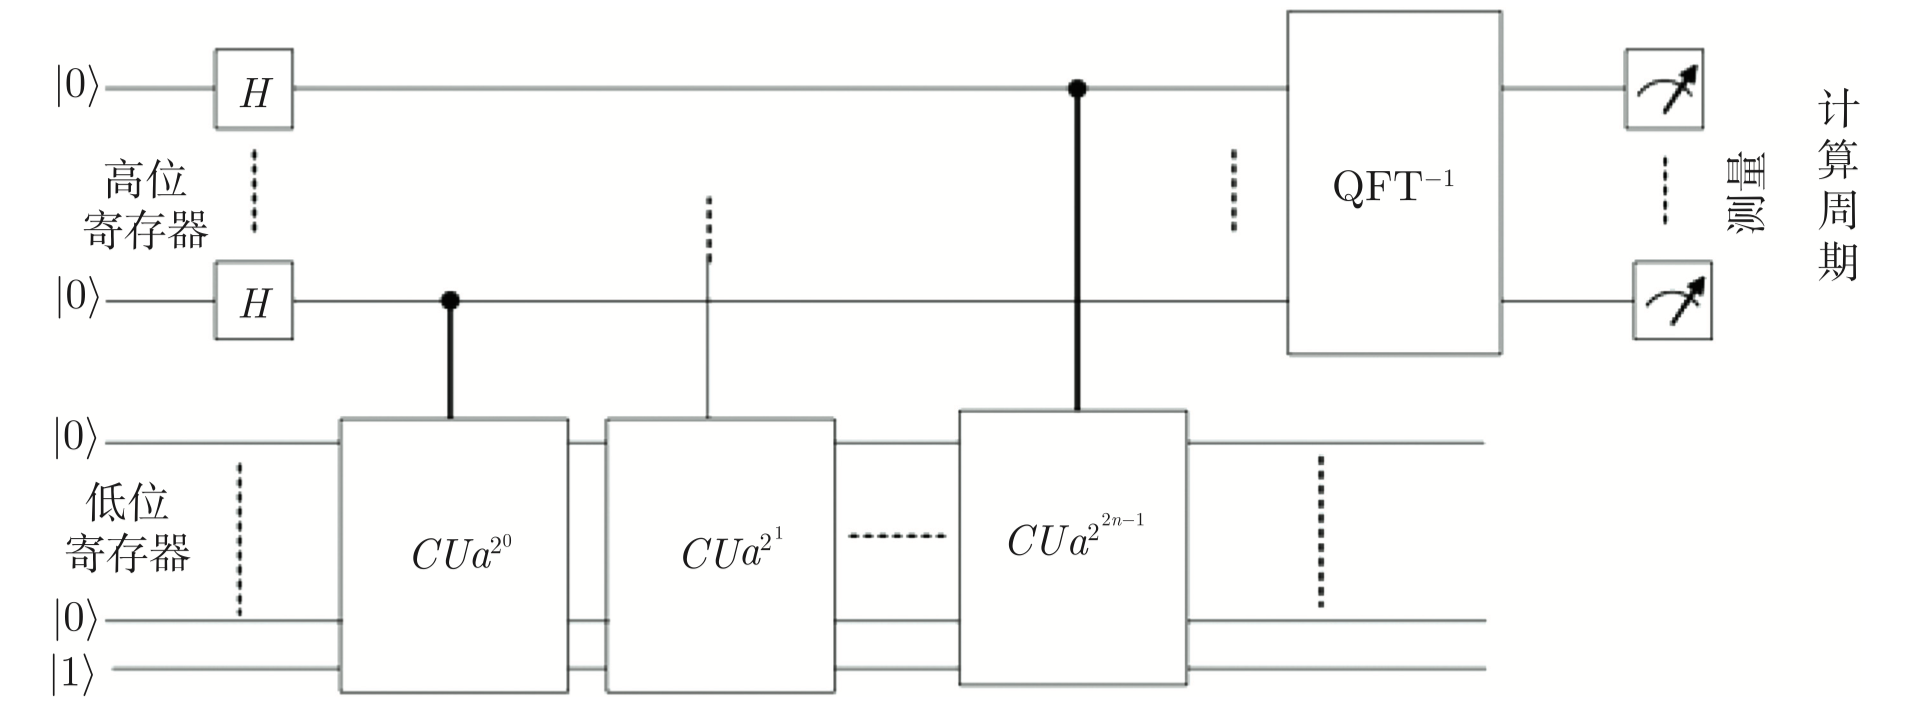
\includegraphics[width =0.8 \textwidth]{figures/态的演化框架图.png}     
    \caption{态的演化框架}
\end{figure}

\newpage
假设 $\mathrm{r} \times \mathrm{m} \approx \mathrm{Q}$, $\mathrm{m}$ 可能是一个大的值。由上述演化可知:经过模指线路, 态呈现一种周期性的规律。
上半部分做 $Q F T^{-1}$ 后:
$$
|i+j r\rangle \rightarrow \frac{1}{\sqrt{Q}} \sum_{k=0}^{Q-1} w^{k(i+j r)}|k\rangle w=e^{\frac{-2 \pi i}{Q}}|\varphi\rangle=\frac{1}{Q} \sum_{i=0}^{r-1} \sum_{j=0}^m \sum_{k=0}^{Q-1} w^{k(i+j r)}|k\rangle|f(i)\rangle
$$
得出共 $r \times Q$ 个态。
此时 $|k\rangle|f(i)\rangle$ 的复振幅:
$$
F_k=\frac{1}{Q} \sum_{j=0}^m w^{k(i+j r)}=\frac{1}{Q} w^{k i} \frac{1-w^{m k r}}{1-w^{k r}}
$$
此时测量 $|\mathrm{k}\rangle$ 态的概率为:

$$
\begin{aligned}
P_k=\sum\limits_{i=0}^{r-1}\left|F_k\right|^2&=\frac{r}{Q^2} \times\left|\frac{1-w^{m k r}}{1-w^{k r}}\right|^2 \\
&=\frac{r}{Q^2} \times \frac{1-\cos (m \theta)}{1-\cos (\theta)} \\
\end{aligned}
$$
$$
\begin{aligned}
\theta&=\frac{k \times r}{Q} \times 2 \pi = s \times 2\pi\\
\end{aligned}
$$
$S$ 为整数时, $P_k$ 取最大值
$$
P_{k \max }=\frac{r}{Q^2} \times m^2 \approx \frac{1}{r}, m \times r \approx Q
$$
由此可知, 可以通过测量概率找到 $\mathrm{r}$ 的关系。
最后测量的 $|k\rangle$, 测量结果满足 $\theta=\frac{k \times r}{Q}$ 为整数或接近整数, 根据 $\frac{k}{Q} \sim \sim \frac{s}{r}$, 对 $\frac{k}{Q}$ 做连分数分解, 可得 $r$ 的周期。

\subsubsection{确认周期}

由于$\frac{k}{Q}$ 是 $\frac{s}{r}$ 的近似, 可以对 $\frac{k}{Q}$ 使用连分数逼近的方法来找到 $\mathrm{r}$,例如:
$$
N=11 \times 7 \,,\, f(x)=3^x \bmod 77\,,\, r=30
$$
Shor 算法中上部分取 14 个量子比特(即 $2 \times 7=14$),$Q=2^{14}$,做连分数逼近得:
\vskip 5pt
\begin{center}
\begin{tabular}{|c|c|c|c|c|c|c|}
    \hline$s / r$ & $k=Q s / r$ & \multicolumn{4}{|c|}{ 连分数逼近 } & 结果 \\
    \hline $1 / 30$ & 546 & $1 / 30$ & & & & 30 \\
    \hline $2 / 30$ & 1092 & $1 / 15$ & & & & 15 \\
    \hline $7 / 30$ & 3823 & $1 / 4$ & $1 / 5$ & $4 / 17$ & $7 / 30$ & 30 \\
    \hline $11 / 30$ & 6007 & $1 / 2$ & $3 / 8$ & $11 / 30$ & & 30 \\
    \hline $11 / 30$ & 6008 & $1 / 2$ & $3 / 8$ & $7 / 19$ & $11 / 30$ & 30 \\
    \hline $17 / 30$ & 9284 & 1 & $1 / 2$ & $4 / 7$ & $17 / 30$ & 30 \\
    \hline
\end{tabular}
\end{center}

\subsection{Shor算法流程}
总结以上内容,Shor算法的流程可概括为以下几步:
\vskip 5pt
1. 随机选择任意数字 $1<a<N$;

2. 计算 $\operatorname{gcd}(a, N)$;

3. 如果 $\operatorname{gcd}(a, N) \neq 1$ 则返回到第一步 ;

4. 当 $\operatorname{gcd}(a, N)=1$ 时, 构造函数 $f(x)=a^x \bmod N$,

\quad 寻找最小周期 $r$, 使得 $f(x+r)=f(x)$;

5. 如果得到找到的 $\mathrm{r}$ 是奇数, 回到第1步;

6. 如果 $a^{\frac{r}{2}}=-1(\bmod N)$, 同样回到第1步, 从新开始选择 $a$;

7. 如果 $a^{\frac{r}{2}} \neq-1(\bmod N)$, 则 $\operatorname{gcd}\left(a^{\frac{r}{2}} \pm 1, N\right)$ 即为所求, 分解完成。

\subsection{Shor算法的代码实现}

\subsubsection{Shor算法代码}
导入依赖的库
\begin{lstlisting}
    from pyqpanda import *
    import matplotlib.pyplot as plt
    import math as m
\end{lstlisting}

绘制数据图所需代码
\begin{lstlisting}
    # 绘制柱状图
    def plotBar(xdata, ydata):
        fig, ax = plt.subplots()
        fig.set_size_inches(6, 6)
        fig.set_dpi(100)

        rects = ax.bar(xdata, ydata, color='b')

        for rect in rects:
            height = rect.get_height()
            plt.text(rect.get_x() + rect.get_width() / 2, height, str(height), ha="center", va="bottom")

        plt.rcParams['font.sans-serif'] = ['Arial']
        plt.title("Origin Q", loc='right', alpha=0.5)
        plt.ylabel('Times')
        plt.xlabel('States')

        plt.show()
\end{lstlisting}

重新组织数据 $quick\, measure$ 的数据
\begin{lstlisting}
    def reorganizeData(measure_qubits, quick_measure_result):
        xdata = []
        ydata = []

        for i in measure_qubits:
            xdata.append(str(i))  # Assuming measure_qubits contains integer indices
            ydata.append(quick_measure_result.get(i, 0))  # Using .get() to avoid KeyError

        return xdata, ydata
\end{lstlisting}

用辗转相除法求最大公约数
\begin{lstlisting}
    def gcd(m, n):
        if not n:
            return m
        else:
            return gcd(n, m % n)
\end{lstlisting}

量子加法器MAJ模块
\begin{lstlisting}
    # a, b, c are single qubits, where a is an auxiliary qubit
    def MAJ(a, b, c):
        circ = QCircuit()
        circ.insert(CNOT(c, b))  # Line 3: Apply CNOT with c as control and b as target
        circ.insert(CNOT(c, a))  # Line 4: Apply CNOT with c as control and a as target
        circ.insert(Toffoli(a, b, c))  # Line 11: Apply Toffoli with a, b as controls and c as target

        return circ
\end{lstlisting}

量子加法器UMA模块
\begin{lstlisting}
    # a, b, c are single qubits

    def UMA(a, b, c):
        circ = QCircuit()
        # Apply Toffoli gate with a, b as controls and c as target
        # Apply CNOT with c as control and a as target
        # Apply CNOT with a as control and b as target
        circ.insert(Toffoli(a, b, c)).insert(CNOT(c, a)).insert(CNOT(a, b))

        return circ
\end{lstlisting}

量子加法器MAJ2模块
\begin{lstlisting}
    # a and b are sets of quantum bits representing specific numbers, here we assume the lengths of a and b are the same
    # c is an auxiliary bit

    def MAJ2(a, b, c):
        if ((len(a) == 0) or (len(a) != len(b))):
            raise RuntimeError('a and b must be equal in length and not equal to 0!')

        nbit = len(a)
        circ = QCircuit()

        # Apply MAJ to the first qubits of a and b, with c as the auxiliary qubit
        circ.insert(MAJ(c, a[0], b[0]))

        # Apply MAJ to the rest of the qubits in sequence
        for i in range(1, nbit):
            circ.insert(MAJ(b[i-1], a[i], b[i]))

        return circ
\end{lstlisting}

量子加法器 由MAJ和UMA模块组成,不考虑进位项
\begin{lstlisting}
    # a and b are sets of quantum bits representing specific numbers, here we assume the lengths of a and b are the same
    # c is an auxiliary bit
    # Note: a stores the result of a+b, while b remains unchanged

    def Adder(a, b, c):
        if ((len(a) == 0) or (len(a) != len(b))):
            raise RuntimeError('a and b must be of equal length and not equal to 0!')

        nbit = len(a)
        circ = QCircuit()

        # Apply MAJ to the first qubits of a and b, with c as the auxiliary qubit
        circ.insert(MAJ(c, a[0], b[0]))

        # Apply MAJ to the rest of the qubits in sequence
        for i in range(1, nbit):
            circ.insert(MAJ(b[i-1], a[i], b[i]))

        # Apply UMA in reverse order to perform the addition
        for i in range(nbit - 1, 0, -1):
            circ.insert(UMA(b[i-1], a[i], b[i]))

        # Apply UMA to the first qubits of a and b, with c as the auxiliary qubit
        circ.insert(UMA(c, a[0], b[0]))

        return circ
\end{lstlisting}

判断是否有进位
\begin{lstlisting}
    # a and b are sets of quantum bits representing specific numbers, here we assume the lengths of a and b are the same
    # c is an auxiliary bit
    # carry is an auxiliary bit used to save the carry bit
    # Note: After this module, the bits in a, b, c remain unchanged, only the carry bit may be changed

    def isCarry(a, b, c, carry):
        if ((len(a) == 0) or (len(a) != len(b))):
            raise RuntimeError('a and b must be of equal length and not equal to 0!')

        circ = QCircuit()

        # Insert MAJ2 module
        circ.insert(MAJ2(a, b, c))

        # Apply a CNOT gate with the last bit of b as control and carry as target
        circ.insert(CNOT(b[-1], carry))

        # Insert the inverse of MAJ2 module to restore the original states
        circ.insert(MAJ2(a, b, c).dagger())

        return circ
\end{lstlisting}

用量子比特来绑定经典数据
\begin{lstlisting}
    # Assuming all bits are initialized to the 0 state

    def bindData(qlist, data):
        check_value = 1 << len(qlist)
        if (data >= check_value):
            raise RuntimeError('data must be less than 2^len(qlist)')

        circ = QCircuit()
        i = 0
        while (data >= 1):
            if (data % 2) == 1:
                circ.insert(X(qlist[i]))

            data = data >> 1
            i = i + 1

        return circ
\end{lstlisting}

常数模加
\begin{lstlisting}
    # qa is a set of qubits bound to classical data and returns the result of the calculation
    # C is the constant to be added
    # M is the modulus
    # qb is a set of auxiliary qubits
    # qs1 is a set of two auxiliary qubits, where qs1[0] is the carry auxiliary qubit, and qs1[1] is the auxiliary qubit used by the MAJ module
    # Note: This module will restore all the auxiliary qubits used

    def constModAdd(qa, C, M, qb, qs1):
        circ = QCircuit()

        q_num = len(qa)

        # Calculate the temporary value for binding
        tmp_value = (1 << q_num) - M + C

        # Bind the temporary value to the auxiliary qubits
        circ.insert(bindData(qb, tmp_value))
        # Perform carry check operation
        circ.insert(isCarry(qa, qb, qs1[1], qs1[0]))
        # Re-bind the temporary value to undo the effect of isCarry
        circ.insert(bindData(qb, tmp_value))

        # Create a temporary circuit for conditional addition
        tmp_circ = QCircuit()
        tmp_circ.insert(bindData(qb, tmp_value))
        tmp_circ.insert(Adder(qa, qb, qs1[1]))
        tmp_circ.insert(bindData(qb, tmp_value))
        # Control the temporary circuit with the carry qubit
        tmp_circ = tmp_circ.control([qs1[0]])
        circ.insert(tmp_circ)

        # Flip the carry qubit
        circ.insert(X(qs1[0]))

        # Create another temporary circuit for adding the constant C
        tmp2_circ = QCircuit()
        tmp2_circ.insert(bindData(qb, C))
        tmp2_circ.insert(Adder(qa, qb, qs1[1]))
        tmp2_circ.insert(bindData(qb, C))
        # Control this circuit with the carry qubit as well
        tmp2_circ = tmp2_circ.control([qs1[0]])
        circ.insert(tmp2_circ)

        # Flip the carry qubit back
        circ.insert(X(qs1[0]))

        # Calculate the value to unbind for the final subtraction
        tmp_value = (1 << q_num) - C
        # Unbind the value for the final subtraction
        circ.insert(bindData(qb, tmp_value))
        circ.insert(isCarry(qa, qb, qs1[1], qs1[0]))
        circ.insert(bindData(qb, tmp_value))
        # Flip the carry qubit for the final operation
        circ.insert(X(qs1[0]))

        return circ
\end{lstlisting}

辗转相除法求模逆
\begin{lstlisting}
    def modreverse(c, m):
        if (c == 0):
            raise RecursionError('c is zero!')

        if (c == 1):
            return 1

        m1 = m
        quotient = []
        quo = m // c
        remainder = m % c

        quotient.append(quo)

        while (remainder != 1):
            m = c
            c = remainder
            quo = m // c
            remainder = m % c
            quotient.append(quo)

        if (len(quotient) == 1):
            return m - quo

        if (len(quotient) == 2):
            return 1 + quotient[0] * quotient[1]

        rev1 = 1
        rev2 = quotient[-1]
        reverse_list = quotient[0:-1]
        reverse_list.reverse()

        for i in reverse_list:
            rev1 = rev1 + rev2 * i
            temp = rev1
            rev1 = rev2
            rev2 = temp

        if ((len(quotient) % 2) == 0):
            return rev2

        return m1 - rev2
\end{lstlisting}

常数模乘
\begin{lstlisting}
    # qa is a set of qubits bound to classical data and returns the result of the calculation
    # const_num indicates the constant to be multiplied
    # M indicates the modulus
    # qs1 auxiliary qubits used for constant modulus multiplication
    # qs2 auxiliary qubits used for constant modulus addition
    # qs3 indicates two auxiliary qubits, where qs3[0] is the carry auxiliary qubit, and qs3[1] is the auxiliary qubit used by the MAJ module
    # Note: This module will restore all the auxiliary qubits used

    def constModMul(qa, const_num, M, qs1, qs2, qs3):
        circ = QCircuit()

        q_num = len(qa)

        for i in range(0, q_num):
            tmp_circ = QCircuit()
            tmp = const_num * pow(2, i) % M
            tmp_circ.insert(constModAdd(qs1, tmp, M, qs2, qs3))
            tmp_circ = tmp_circ.control([qa[i]])
            circ.insert(tmp_circ)

        # State swap
        for i in range(0, q_num):
            circ.insert(CNOT(qa[i], qs1[i]))
            circ.insert(CNOT(qs1[i], qa[i]))
            circ.insert(CNOT(qa[i], qs1[i]))

        # Calculate the modular multiplicative inverse using the extended Euclidean algorithm
        Crev = modreverse(const_num, M)

        # Apply the modular multiplication with the modular multiplicative inverse
        tmp2_circ = QCircuit()
        for i in range(0, q_num):
            tmp = Crev * pow(2, i)
            tmp = tmp % M
            tmp_circ = QCircuit()
            tmp_circ.insert(constModAdd(qs1, tmp, M, qs2, qs3))
            tmp_circ = tmp_circ.control([qa[i]])
            tmp2_circ.insert(tmp_circ)

        # Inverse the circuit to undo the operations
        circ.insert(tmp2_circ.dagger())

        return circ
\end{lstlisting}

常数模指
\begin{lstlisting}
    # qa is a set of control qubits
    # qb stores the calculation result
    # base indicates the exponential base
    # M indicates the modulus
    # qs1 auxiliary qubits used for constant modulus multiplication
    # qs2 auxiliary qubits used for constant modulus addition
    # qs3 indicates two auxiliary qubits, where qs3[0] is the carry auxiliary qubit, and qs3[1] is the auxiliary qubit used by the MAJ module

    def constModExp(qa, qb, base, M, qs1, qs2, qs3):
        circ = QCircuit()

        cqnum = len(qa)

        temp = base

        for i in range(0, cqnum):
            # Perform constant modulus multiplication controlled by the i-th control qubit from qa
            circ.insert(constModMul(qb, temp, M, qs1, qs2, qs3).control([qa[i]]))
            # Update the base by squaring it
            temp = temp * temp
            # Apply modulus to the updated base
            temp = temp % M

        return circ
\end{lstlisting}

量子傅里叶变换
\begin{lstlisting}
    # qa is a set of control qubits
    # qb saves the calculation result
    # base indicates the exponential base
    # M indicates the modulus
    # qs1 auxiliary qubits used for constant modulus multiplication
    # qs2 auxiliary qubits used for constant modulus addition
    # qs3 indicates two auxiliary qubits, where qs3[0] is the carry auxiliary qubit, and qs3[1] is the auxiliary qubit used by the MAJ module

    def constModExp(qa, qb, base, M, qs1, qs2, qs3):
        circ = QCircuit()

        cqnum = len(qa)

        temp = base

        for i in range(0, cqnum):
            # Perform constant modulus multiplication controlled by the i-th qubit from qa
            circ.insert(constModMul(qb, temp, M, qs1, qs2, qs3).control([qa[i]]))
            # Square the temporary base and apply modulus to it
            temp = (temp * temp) % M

        return circ
\end{lstlisting}

Shor算法主体代码
\begin{lstlisting}
    # base indicates the exponential base
    # M indicates the number to be factored

    def shorAlg(base, M):
        if ((base < 2) or (base > M - 1)):
            raise ValueError('Invalid base!')

        if (gcd(base, M) != 1):
            raise ValueError('Invalid base! base and M must be mutually prime')

        binary_len = 0
        while M >> binary_len != 0:
            binary_len = binary_len + 1

        machine = init_quantum_machine(QMachineType.CPU_SINGLE_THREAD)

        qa = machine.qAlloc_many(binary_len * 2)
        qb = machine.qAlloc_many(binary_len)

        qs1 = machine.qAlloc_many(binary_len)  # Auxiliary qubits for constant modulus multiplication
        qs2 = machine.qAlloc_many(binary_len)  # Auxiliary qubits for constant modulus addition
        qs3 = machine.qAlloc_many(2)  # Auxiliary qubits for carry in addition

        prog = QProg()

        # Initialize the first qubit of qb to 1
        prog.insert(X(qb[0]))

        # Apply Hadamard gate to all qubits in qa
        prog.insert(single_gate_apply_to_all(H, qa))

        # Apply the controlled modular exponentiation
        prog.insert(constModExp(qa, qb, base, M, qs1, qs2, qs3))

        # Apply the inverse quantum Fourier transform to qa
        prog.insert(qft(qa).dagger())

        # Directly run the quantum program
        directly_run(prog)

        # Measure the result from qa
        result = quick_measure(qa, 100)

        # Print the measurement result
        print(result)

        # Reorganize the measurement result for plotting
        xdata, ydata = reorganizeData(qa, result)

        # Plot the histogram of the measurement results
        plotBar(xdata, ydata)

        return result
\end{lstlisting}

主程序
\begin{lstlisting}
    if __name__ == "__main__":
        base = 7
        N = 15
        shorAlg(base, N)
\end{lstlisting}

\subsubsection{模拟结果分析}

在本节中,我们使用了Shor算法对整数N=15进行因数分解模拟,底数a取7。在对Shor算法的量子电路进行代码实现后,我们得到了4种量子比特串的测量结果:
\newpage

\begin{figure}[!htbp]     
    \centering     
    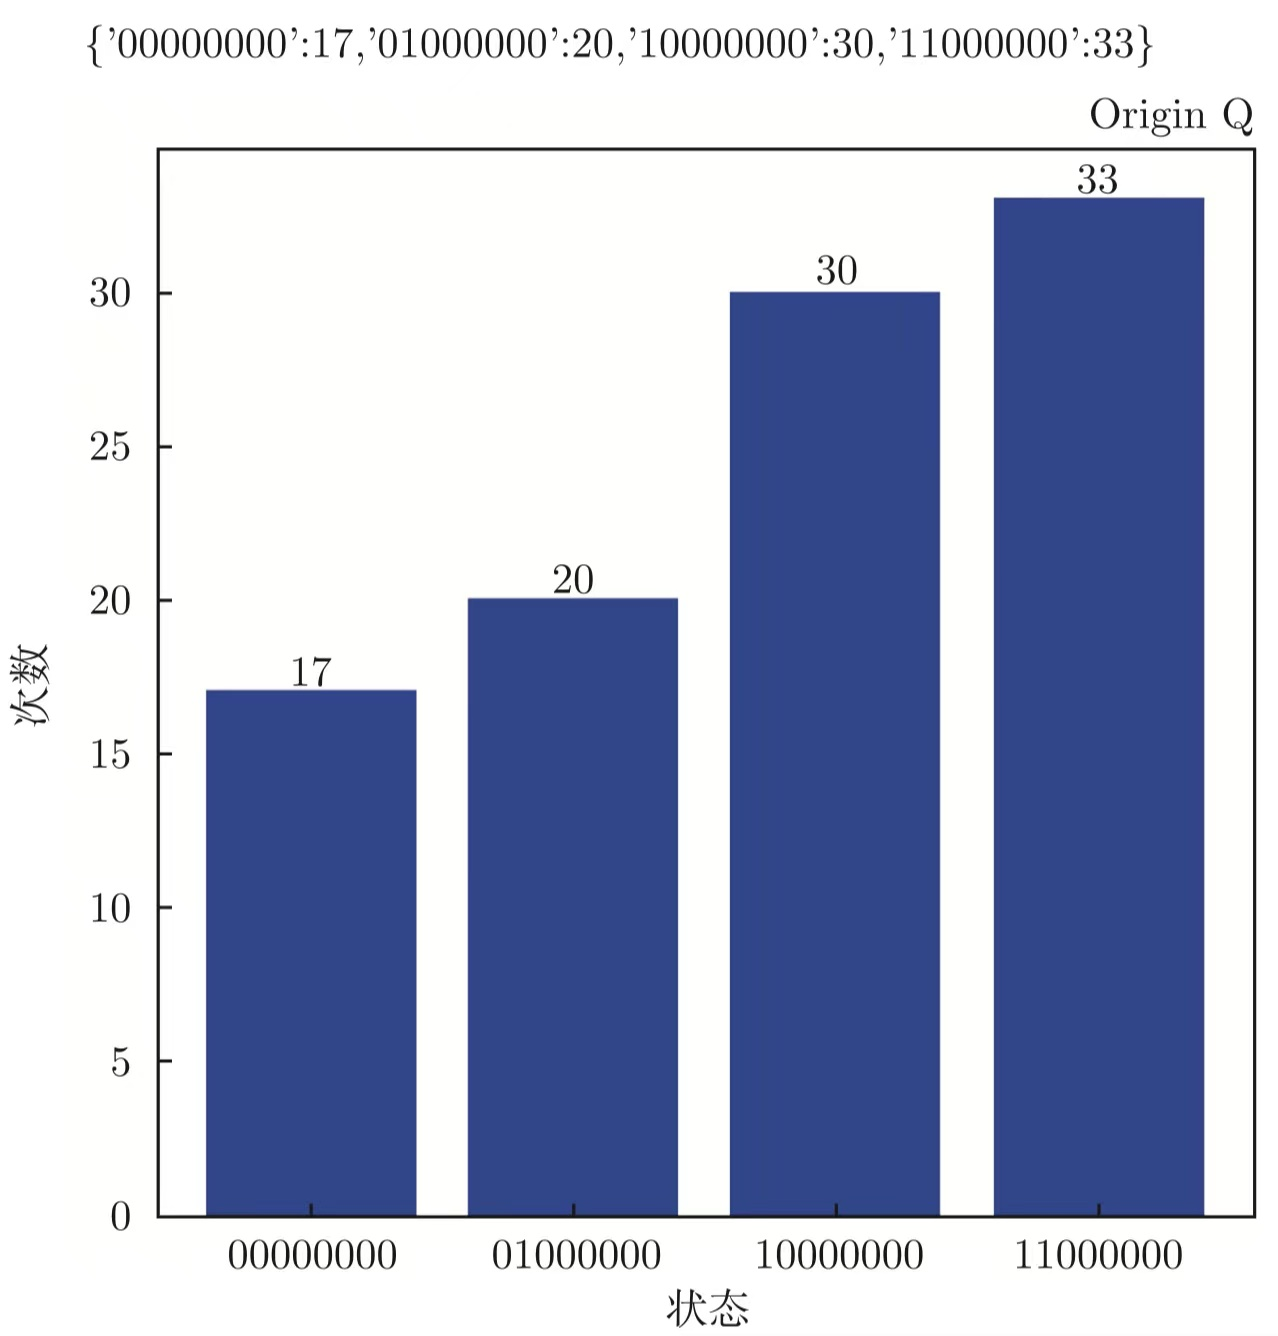
\includegraphics[width =0.7 \textwidth]{figures/结论.jpeg}     
    \caption{Shor算法模拟结果(分解N=15,a取7)}
\end{figure}

\noindent
这些字符串是qa量子寄存器的测量结果,每个结果都分别对应于一个特定的二进制数,转化为十进制为0,1,2,3.
3的测量结果出现的次数最多,因此我们可以认为3是最可能的结果。根据节3.3.5的方法,取k=3,本次模拟取了8个量子比特,对应的$Q=2^{8/2}=16$,故$\frac{k}{Q}=\frac{3}{16}$. 
对$\frac{3}{16}$做连分数分解,得$r$的周期为4,故$N=15$的两个质因数为:
$$
gcd(7^{4/2}+1, 15)=gcd(50, 15)=5
$$
$$
gcd(7^{4/2}-1, 15)=gcd(48, 15)=3
$$
模拟成功。

\vskip 50pt
\textit{尽管现在很多程序库都有了Shor量子算法包,只需简单掉包即可实现素数分解。但本文从较为底层的量子门级别展开分析并编写代码,实现了Shor算法的模拟,并成功地对整数N=15进行了因数分解。量子计算仍是一个新兴的领域,我十分期待在未来的研究中能够更深入地探索量子计算的奥秘。}







\end{document}